\chapter{Methodology \& Numerical Simulation}
\label{ch:numsim}

% Brief summation of computational work
Observational astrophysics is a curious field based on snapshots.
The universe can be thought of as a near-infinite number of laboratory experiments, that are viewed from the astronomer from a fixed perspective, through a very large telescope.
Most phenomena too, evolve over incredibly long timescales, it may in some cases take the entire lifetime of a researcher to collect enough information on a single system - in other cases, they may be long dead before their predictions can be validated.
Despite this, by observing many systems at once, we can overcome this limit, piecing together the properties and formation of phenomena from a thousand disparate snapshots in space and time.
This kind of ``natural parallelisation'' works, to a point, and where it doesn't numerical simulation can step in.
While a comparatively recent method of research, and only within the last two decades has computing hardware been up to the task of simulating 3D environments, numerical simulation is vital for gaining insight on regions that are hard to observe.
The WCR of a CWB system is extremely difficult to observe, and as such, we turn to simulation in order to understand the region better.
Unfortunately, it is also comparatively difficult to simulate as well, as we will discuss.

% Why is this it's own chapter?
As mentioned in the introduction to this thesis, theoretical astrophysics straddles two complex fields, astrophysics and computer science.
To this end, while we have discussed the underlying physics and physical phenomena of this project, we have so far neglected to cover the simulationist aspects of this work.
Some astrophysicists reading this thesis may be unfamiliar with the computational side of the work, and vice versa for computer scientists - as such it is best to describe both in detail.
Furthermore, discussing our methodology in its own section consolidates it and makes it easier for the reader to understand and replicate it.
% Breakdown of chapter, what this involves
This chapter primarily deals with detailing numerical simulations, in particular how they work and why they are being utilised, as well the development and implementation of a CWB model inside the \athena{} hydrodynamical code.
We also detail our attempts to implement radiative cooling, as well as our advected scalar dust model, \bidmas.

\section{The History \& Mathematics of Numerical Simulations}
\label{sec:numerical-math}
\label{sec:numsim}

% Numerical solvers/Riemann problems
In astrophysical fluid dynamics, the most fundamental of equations are the Euler equations.
These are a specific case of the more general Navier-Stokes equations of fluid dynamics, covering the case of an inviscid fluid lacking thermal conductivity.
These properties make the equations ideal for application to astrophysical fluids.
At vast length scales the aggregate properties of a collection of molecules in near vacuum are essentially in-line with what is predicted by inviscid fluid dynamical equations.
Because of the general lack of physical contact, being both rare and fleeting, the influence of thermal conduction and convection on the fluid are essentially ruled out.
Astrophysical fluids at first appear strange and unintuitive compared to the more familiar fluid dynamics that we have an almost innate understanding of as human beings.
However, if one zooms out enough and starts thinking in terms of parsecs and astronomical units, some similarities do appear, such as instabilities, turbulence and shocks.

In a one-dimensional adiabatic case, with a fluid of density $\rho$, a velocity of $u$, a fluid pressure of $P$ and a total energy, $E$, the Euler equations take the form:

\begin{subequations}
  \begin{align}
    \frac{\partial \rho}{\partial t} & + \frac{\partial}{\partial x} (\rho u) = 0 ,\\
    \frac{\partial \rho u}{\partial t} & + \frac{\partial}{\partial x} (\rho u^2 + P) = 0 ,\\
    \frac{\partial E}{\partial t} & + \frac{\partial}{\partial x} \left[ u(E+P) \right] = 0 .
  \end{align}
\end{subequations}

\noindent
As the Euler equations are a non-linear series of partial differential equations, no general analytical solution exists, to make it worse, numerical solutions aren't exactly easy either.
% Godunov method and other exact methods
The basest method of numerically solving such problems is Godunov's scheme \parencite{godunov_difference_1959}; this scheme is a finite-volume method wherein the problem is split into a series of cells, with a Riemann problem between the interfaces of each cell (Fig. \ref{fig:riemann}), an approximate solution to the Euler equations can then be made by solving all of these Riemann problems in sequence and integrating across a time-step, $dt$.
The problem can be simulated and solved by marching through many time-steps, until the required advection time is achieved.
This provides a first-order accurate approximation in a more general form, compared to the otherwise intractable set of PDEs. 
Whilst this piecewise method of solving many thousands of Riemann problems may provide a more generalised method of calculating fluid dynamics, performing it by hand would invoke a terrible strain on a mathematician's wrists.

\begin{figure}[ht]
  \centering
  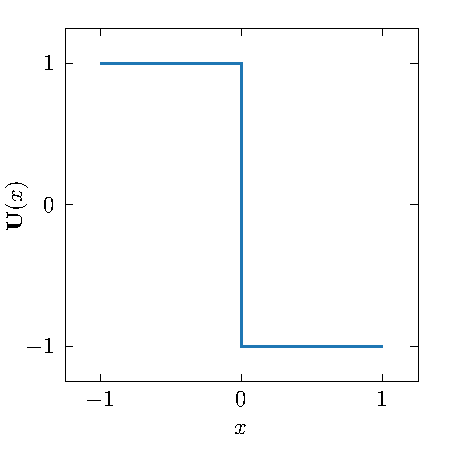
\includegraphics[]{assets/riemann-interface/riemann.pdf}
  \caption[Initial conditions of a Riemann problem]{The initial conditions of a Riemann problem, where $\mathbf{U}$ is a conserved variable.}
  \label{fig:riemann}
\end{figure}

Godunov's scheme however, coincided with the burgeoning field of computer science.
Computers are extremely well suited to this type of calculation, and can solve Riemann problems many orders of magnitude faster than a mathematician with repetitive strain injury.
Solving a higher-dimensional problem is a conceptually trivial extension to the original 1-D problem.
In the 2-D case the number of interfaces increases to 4, with each interface being the analogous to each side of a square or rectangle, while in the 3-D case the interfaces can be thought of as the 6 faces of a cuboid.
As such, the general formulation of the Euler equations becomes:

\begin{equation}
  \frac{\partial \mathbf{U}}{\partial t} + \nabla \cdot \left[ \mathbf{F}(\mathbf{U}) \right] = 0 ,
\end{equation}

\noindent
where $\mathbf{U}$ is a vector of conserved variables and $\mathbf{F}(\mathbf{U})$ is a vector of the corresponding fluxes of the conserved variables:

\begin{equation}
  \mathbf{U} = 
  \begin{bmatrix}
    \rho \\
    \rho u \\
    E
  \end{bmatrix}
  , ~
  \mathbf{F}(\mathbf{U}) =
  \begin{bmatrix}
    \rho \boldsymbol{u} \\
    \rho u \boldsymbol{u} + P \\
    \boldsymbol{u}(E + P)
  \end{bmatrix} .
\end{equation}

In practise however, solving higher-dimensional problems are significantly more computationally intensive, due to the increased number of interfaces and the drastically increased number of cells required to simulate the problem.

% HLLC method, as used in project

Initial methods involved exact solutions to the Riemann problems, however, this is a time consuming method.
Instead, approximate methods were developed to improve numerical performance.
However, early methods were less exact, and could not preserve the contact surface, these methods were also markedly less stable, limiting their effectiveness.
Later models, such as the Harten-Lax-van Leer-Contact (HLLC) solver \parencite{toroRestorationContactSurface1994} are approximate solvers that offer a similar order of accuracy to the exact solution, while being significantly faster than the exact solution and more numerically stable than earlier approximate solvers.
As such, this method is commonly used in hydrodynamical codes, and is used in this project as one of the methods included in \athena.

% Piecewise methods
Godunov's method is commonly used as a base for higher-order extensions, which employ methods to interpolate and reconstruct the flow between the interfaces of each Riemann problem.
Piecewise linear linearly interpolates fluxes between cells to reconstruct the cell interfaces, and is generally considered to be significantly more versatile than a simple piecewise \parencite{vanleerUltimateConservativeDifference1979}
The piecewise parabolic method performs a parabolic interpolation step instead, this is generally more accurate for a smooth and continuous flow, but most schema must account for and detect discontinuities
\parencite{colella_piecewise_1984}.
Throughout this project we use the piecewise linear method, which is the default for \athena{} and \mg{}.
This was found to be more than suitable for our work.

% Integration
In order to solve the problem, the fluxes along each cell interface are integrated across time, in the case of this project, a third-order accurate Runge-Kutta (RK) method is used.
% Courant number
The integration timestep is typically much smaller than the 
Overall, with $n$ spatial dimensions and 1 time dimension, it is clear how computationally intensive these simulations are.
This timestep must be carefully calibrated to ensure that the duration of the integration step is less than the time taken for a fluid to advect through to an adjacent cell.
If a clump of gas, for instance, travels across two adjacent cells in a single timestep, the interaction occurring in the middle cell would be lost, and unphysical behaviour would occur.
This is especially a problem in the case of highly supersonic flows, where the fluid is moving extremely fast.
This problem is further compounded with multiple dimensions, which must all be accounted for in a similar manner.
The Courant-Friedrichs-Lewy condition determines that the maximum integration time should not be higher than the time taken for a fluid to advect between adjacent cells in a numerical grid.
This condition defines a value $C$, or the CFL number, and is the ratio between the wave propagation speed, $u$, and the grid speed, $\Delta x / \Delta t$.
For multiple dimensions, the CFL number is calculated with the formulae

\begin{equation}
  C = \Delta t \left(\sum^n_{i=1} \frac{u_{x_i}}{\Delta x_i}\right) ,
\end{equation}

\noindent
where $\Delta t$ is the timestep, $u_{x_i}$ is the velocity of the fluid along dimension $i$ and $\Delta x_i$ is the cell spacing for dimension $i$ \parencite[Ch.~5]{toro_riemann_2013}.
Hydrodynamical codes typically allow the user to define $C$ such that the code can calculate the necessary timestep.
For instance, in the case of a three-dimensional problem, $\Delta t$ is found to be

\begin{equation}
  \Delta t = \frac{C}{(u_x/\Delta x) + (u_y/\Delta y) + (u_z/\Delta z)}.
\end{equation}

\noindent
For an explicit time-integration problem such as numerical simulation, the value of $C$ is typically $\leq 1$, with the timestep decreasing with additional dimensions for a given value of $C$.
For 3-dimensional problems in this work, we typically start at $C = 0.15$, and decrease if necessary.

Numerical simulations - whilst extremely processing intensive - are a class of problems that are considered to be \emph{embarrassingly parallel}.
A hydrodynamical problem can be divided into a series of smaller problems and solved independently for a common timestep.
These numerical grids must be checked for concurrency at the interfaces between grids, which introduces some overhead to the parallelism, but on the whole is significantly faster than a single-threaded method.
This subdivision can be performed through striping along one of the dimensional axes, with stripes distributed to a specific processor (performed by \mg{} and \texttt{VH-1}).
Another method for parallelism is reducing the entire problem to a series of blocks that are solved in parallel (performed by \athena). 
Other enhancements to numerical simulation include mesh refinement, which is covered in more detail in Section \ref{sec:refinement}.

\section{The Purpose of Numerical Simulations}
\label{sec:numerical-purpose}

% Why are they useful in general
Numerical simulation, thanks to its generalised but calculation-intensive approximation of partial differential equations, has an enormous range of uses - especially in the field of astrophysics.
In particular, numerical simulations excel in modelling large timescales and regions that are difficult or impossible to observe.
The laws of physics have remained fairly consistent over the last 13.8 billion years\footnote{With some earlier exceptions, see cosmological inflation.}, and as such simulations have been performed of the early universe.
The dynamics and collapse of the universe into filaments and galaxies provides our only continuous look into the long-term evolution of the universe.
Regions that undergo too much extinction from dust or that are too distant to observe can be simulated, as long as a reasonable estimation of the initial system parameters can be made.
Numerical simulation, in a sense, fills in the gaps and weaves together the many snapshots of the universe we can make from our lone vantage point in our more uneventful pocket of the cosmos.

I must stress, however, that this is not me screwing my simulationist hat firmly onto my head and claiming that theoretical astrophysics is inherently superior to observational.
Whilst an immensely versatile and useful weapon in an astrophysicists arsenal, numerical simulations are almost entirely reliant on the understanding of the laws of physics as we know them.
The remainder of that reliance rests on the ability of the programmer, and on the assumptions and initial conditions of the simulation.
In the case of poor assumptions and parameters, we find that the computer scientist idiom of ``garbage input, garbage output'' begins to apply.

% Why are they useful in the context of a colliding wind binary problem

Colliding wind binaries are a class of astrophysical phenomena that have a particularly strong dependence on numerical modelling in order to study them.
The WCR is extremely difficult to observe for a variety of reasons:

\begin{itemize}
  \item The nearest WCR is over \SI{1}{\kilo\parsec} away, and the structure is comparatively small, on the order of a few \si{\au}.
  \item The structure can also be obscured by the parent stars, which are typically brighter in the optical and UV spectra.
  \item The WCR is extremely dense, leading to significant reddening and extinction.
  \item Dense winds from the WR star can also worsen extinction.
\end{itemize}

\noindent
Observation of the large-scale structure of the WCR is possible with current telescopes, as is clear observation of the surrounding dust cloud (such as in the case of Apep, see \cite{callinghamAnisotropicWindsWolf2019}).
Observation of the small dust forming region is far more difficult.
In most cases, a telescope with an angular resolution $<50\,\si{\micro\arcsecond}$ would be required to resolve the region, ruling out even the highest resolution instrumentation.
Thus, numerical simulation is a requirement.
Implementation of a dust model in order to analyse how dust growth occurs within the region can also be performed and compared to observational estimates.
Radiative transfer models can also be used to model the dust production rate of these systems, however this was not feasible in the constraints of this projects timescale.

% Why are colliding wind binary systems such a pain to solve
CWB systems, however, are difficult to \emph{simulate} as well!

Numerical simulations are vastly simplified by reducing the number of dimensions.
Single object systems can be reduced to 1-D spherically symmetric or 2-D cylindrical axisymmetric representations.
This is the case in earlier simulations of supernovae and jets.
Simulations of CWB systems are possible with cylindrical symmetry, but inclusion of orbits will negate the effects due to orbital motion, such as pinwheel formation.
The apex of the WCR must be properly resolved from either of the stars, in the case of systems with imbalanced winds this can result in a cell width, $\Delta x$, of $<1/100^{\text{th}}$ of the orbital separation\footnote{This value is derived from experimentation, but is a good place to start.}.
Ideally, to simulate a CWB system, it is preferable to simulate a large domain, typically \SI{100}{AU} to \SI{1000}{AU}.
This further increases the number of cells required to simulate the system.
Finally, the extreme degree of cooling in the post-shock WCR can render the simulation unstable, requiring robust cooling techniques or very small timesteps to ensure stability.
All of these factors enact a significant computational cost, requiring a large number of cores to effectively simulate the systems.
Fortunately, mesh refinement techniques can improve this situation by drastically reducing the number of cells that need processing, simplifying our problem from \textit{impossibly} intensive to merely \textit{extremely} intensive.

\section{The \mg{} hydrodynamical code}
\label{sec:mgcode}

% briefly cover MG hydrodynamical code, since this was used for the first half of this work before adopting a more modern hydro code

Initially this project intended to use the \mg{} hydrodynamical code, as CWB systems had already been simulated, with the resultant code being readily available in the department.

\mg{} is comparatively easy to use and understand, and had a number of features that were useful for this project, such as MPI parallelism and adaptive mesh refinement.
It was initially estimated that it would take little more than a year to implement the dust and cooling models; large-scale simulations on the ARC3 and ARC4 computers would be underway mid-way through the second year of research.

How wrong we were.

% why we didn't use it in the end

Unfortunately the advected scalar dust model never adequately worked
This model either produced dust rates measurable in grams per year, or the simulation rapidly converted all wind into dust.
Attempts to implement the dust model through modification of the conserved variables or through a rate-based source function were made, with many different implementation attempts.
None of these panned out, resulting in a large amount of work being discarded.
Using strict constraints to prevent rigorous dust production resulted in strange looking systems, that did not behave as observations suggested.
Furthermore, building a model that relies on dozens of constraints based on limited empirical data is rarely a good model, and is analogous to building a clock without a driving mechanism - such that it is at least right twice a day.

In addition to incompatibility with the dust model, numerous technical issues compounded this work.
Mapping the wind onto the CWB also proved difficult when combined with AMR, as the provided implementation of wind remapping required a circular region with a radius of 3 coarse cells.
In order to get the required separation for systems with close orbits, a very high coarse resolution would be required, massively increasing memory usage and removing the benefits of mesh refinement.
using a source function for wind mapping allowed for more refined cells to be used.
However, this could also produce artefacts at level transitions, while also producing wind temperatures in the order of \SI{1e7}{K}.

In general, while being very extensible in terms of being able to implement a problem generator fairly easily, low-level manipulation of the code was found to be extremely difficult due to limited documentation and a complex, linked-list grid structure.
Writing workarounds and fixes to the issues described was very time-consuming, slowing progress in the project significantly.
Iteration time was also extremely long, requiring multiple hours to run a simulation to determine if the fixes worked.
Debugging was rendered difficult by the use of OpenMPI, and the general structure of the code rendered the setting of breakpoints difficult even in the single-threaded case.
Finally, the numerical integrator was found to be unstable in the face of extremely radiative cooling environments, complex multi-step cooling processes were considered and implemented, but even these could not handle such rapid cooling without breakdown if a reasonable Courant number was to be used.
The solution to this was to artificially limit cooling to a fraction of the energy in the cell per timestep.
This reduced the simulation accuracy, and resulted in much slower cooling within the post-shock WCR\footnote{I understand, reader, that this section reads like a series of complaints\ldots This is because it is. I recommend that you humour me, as attempting to debug \mg{} ate up more than two years of my life and was the direct cause of many, \textit{many} sleepless nights. Thankfully this is the last time we will ever speak of it, unless you and I share a pint or two at a local pub.}.

In the end, the decision was made to switch from \mg{} to the then-new \athena{} hydrodynamical code.
This decision was made in mid-2020, by the end of 2020 the problem generators were built, the necessary modifications to the underlying code of \athena{} were completed and the dust model was fully implemented.
What began next was a frenzy of activity in order to assure that there was sufficient data to complete this project in time.

\section{The \athena{} hydrodynamical code}
\label{sec:athenapp}

The \footlink{\athena{}}{https://github.com/PrincetonUniversity/athena} hydrodynamical code was found to be a much more suitable fit for this project.
\athena{} is a total re-write of the older Athena MHD code in \texttt{C++} with a focus on implementing Adaptive Mesh Refinement, source code clarity, modularity, and improved performance \parencite{stoneAthenaAdaptiveMesh2020}.
This clarity and modularity allowed us to port over our dust model from \mg{} to \athena{} in a few months.
The hydrodynamical problem is defined at compile time, and as such ensures there is no overlapping code from other problem generator codebases.
As such we were able to rapidly iterate and build a new version extremely quickly.

Multiple time-integration and spatial reconstruction methods have been implemented into \athena{}.
Time-integration method vary from a computationally simple \nth{2} order van Leer \parencite{vanleerUltimateConservativeDifference1979} method to strong stability preserving methods \parencite{ruuthHighOrderStrongStabilityPreservingRungeKutta2005} to super time-stepping Runge-Kutta-Legendre \parencite{meyerStabilizedRungeKuttaLegendreMethod2014} methods.
Changing of the time-integration method can be implemented without recompilation, and can even be changed upon restart of an in-progress simulation.
This was useful in the case of simulations, where lowering the CFL number of the simulation did not improve stability.
For this project, either the \nth{3} order accurate strong stability preserving Runge-Kutta method (\texttt{rk3}) or the \nth{4} order accurate, five-stage, 3 register, SSPRK method was utilised (\texttt{ssprk5\_4}), depending on the instability of the simulation.
The \texttt{rk3} method was found to be more than twice as fast as the \texttt{ssprk5\_4} method in the case of a CWB system (Table \ref{tab:rkssprkcomparison}), though could crash in the case of rapid cooling and dust production.
In the case of simulation crashing multiple times, the simulation would be run from the nearest checkpoint using \texttt{ssprk5\_4}. 
\athena{} must be recompiled for the specific spatial reconstruction method, as the number of overlapping ``ghost'' cells needs to be defined at compile-time.
For this project the piecewise linear method was utilised, as this was sufficiently fast and stable.
The Riemann solver can also be changed at compile-time, however this was left to the default solver, the Harten-Lax-van Leer-Contact (HLLC) solver \parencite{toroRestorationContactSurface1994}.

\begin{table}[h]
  \centering
  \begin{tabular}{cccc}
  \hline
  Integrator & Elapsed Time & Relative Time & $\tau_f$ \\ \hline
  \texttt{rk3}       & \SI{1444.6}{\second} & 100.0\% & \SI{5.467E+05}{\second}\\
  \texttt{ssprk5\_4} & \SI{2352.4}{\second} & 163.1\% & \SI{5.542E+05}{\second}\\ \hline
  \end{tabular}
  \caption{Time elapsed}
  \label{tab:rkssprkcomparison}
\end{table}


% Meshblock system

\athena{} has an exceptionally fast parallel performance, with our tests indicating a parallel fraction of $>98\%$ (See Appendix \ref{app:parallelism}).
Large scale weak-scaling testing by \textcite{stoneAthenaAdaptiveMesh2020} found an 80\% parallel efficiency after overhead and memory bandwidth bottlenecks.
Parallelism through block-based division of the numerical problem is utilised, dividing the problem into a regular array of sub-volumes containing a defined number of cells along $X\times Y \times Z$ cells.
This is referred to as a ``meshblock'', and is distributed to a processor available to a programme to be solved.
Meshblocks are encoded in an octree structure, as the relationship between parent and child blocks must be preserved in order for mesh refinement to work correctly.
In comparison to \mg{}, the linked-list method is comparatively slow on modern hardware, as larger processor caches can store arrays contiguously, while linked-lists require fetching elements from RAM.
\athena{} uses \texttt{OpenMP} and \texttt{OpenMPI} for parallelism.
Both can be leveraged in a hybrid shared/distributed memory parallelism schema, and scales well to the thousands of available processing cores on ARC4.
% Ghost cells
To prevent numerical errors from occurring between the interfaces between meshblocks, ``ghost cells'', or cells from adjacent meshblocks copied into the current meshblock, are used.
In this work, the two outermost layers of cells in a meshblock are distributed to the processing nodes solving adjacent meshblocks.
% Briefly discuss parallel performance
Typically, \num{128} cores were used for each simulation, as this represented a good trade-off in processing throughput and node availability, as ARC4 is a heavily utilised resource.

\section{Mesh Refinement}
\label{sec:refinement}

A problem previously discussed with modelling CWB systems is that the apex of the WCR is extremely large relative to the system itself.
As such we must resolve an area approximately 4-5 orders of magnitude smaller than the overall domain of the simulation.
For a 3-D simulation this results in an effective resolution of $10^9$ cells or higher.
In the case of the more ambitious simulations in this project, a region approximately \SI{1000}{\au} was defined, with an effective resolution of approximately \num{1.07e12} cells.
This amount of data is difficult to \emph{store}, let alone compute, and was far beyond the capabilities of any computing resources available to the project.
As the spacing between cells is reduced, the maximum stable timestep decreases as well, in accordance with the CFL condition, worsening the computational requirements.

\begin{figure}[h]
  \centering
  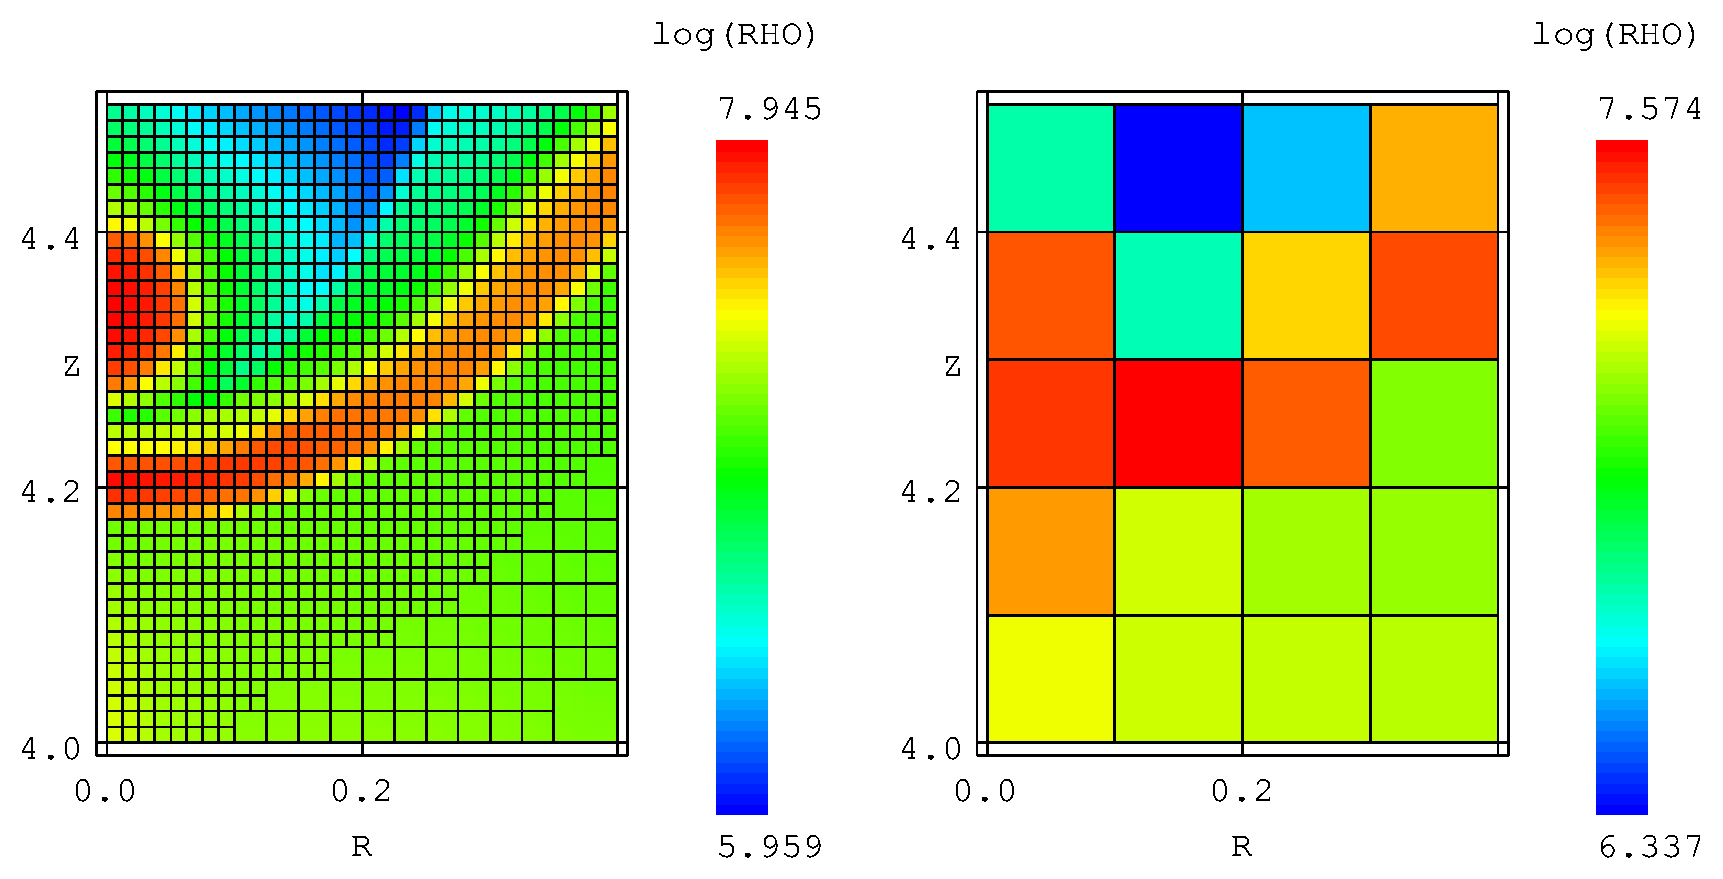
\includegraphics[width=5in]{assets/mergecellc.pdf}
  \caption[Adaptive mesh refinement comparison]{An example of adaptive mesh refinement in the \texttt{MG} hydrodynamical code around the OB star in a colliding wind binary problem using cylindrically symmetric co-ordinates. With AMR the WCR is properly resolved, while without the system cannot adequately resolve the WCR.}
  \label{fig:mgrefine}
\end{figure}

Algorithms such as adaptive mesh refinement, first discussed by \textcite{bergerAdaptiveMeshRefinement1984} and expanded upon by \textcite{bergerLocalAdaptiveMesh1989}, start with a much lower resolution ``coarse'' mesh, and refine specific parts of the simulation.
At each step each cell is tested against pre-defined conditions, such as the proximity to an object in the simulation, a conserved parameter or the truncation error between lower and higher level.
If the cell passes these tests, it is flagged for refinement.
Truncation error in particular, is a useful general purpose refinement criteria, and is used as the refinement mechanism in \mg (Fig. \ref{fig:mgrefine}).
Refinement occurs at the end of a simulation step, splitting the cell in half along each simulation dimension.
The effective dimensional resolution of a simulation with $n$ levels is given by the formulae

\begin{equation}
  x\rms{AMR} = x\rms{coarse} \times 2^{n-1},
\end{equation}

\noindent
where $x\rms{coarse}$ is the number of cells along the dimensional axis at the lowest level, $n=0$.
In the case of a CWB simulation, this would ensure the region inside the orbit of the star and the WCR would be correctly resolved.
Care must be taken not to over-refine the simulation or to rapidly refine and de-refine a region.
The former can be mitigated by defining a maximum refinement level, while the latter can be mitigated by defining a minimum number of timesteps required for a cell to be repeatedly flagged for refinement and de-refinement.
% //TODO Check with Julian 
Another issue with this method is multiple refinements per timestep for a cell, which can cause the simulation to crash.

\begin{figure}[ht]
  \centering
  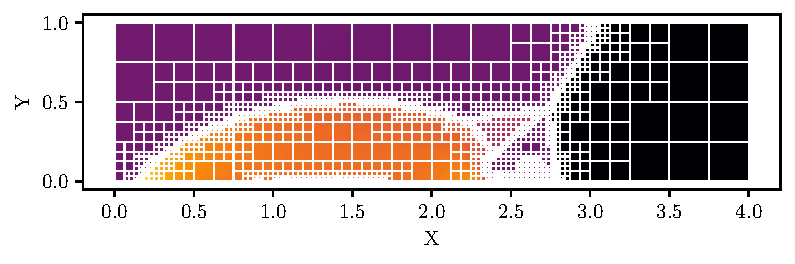
\includegraphics{assets/refinement/dmach/plot.pdf}
  \caption[\athena{} adaptive mesh refinement example]{An example of AMR usage in athena. A double Mach reflection test with a meshblock size of $16 \times 16$ cells and 5 levels. Meshblock interfaces are represented by grid lines.}
  \label{fig:athena-amr-example}
\end{figure}

\athena{} implements mesh refinement by refining and de-refining meshblocks.
The refined blocks are stored as children of the coarser, higher level parent meshblock in the meshblock octree.
% Testing
In order to test the efficacy of this implementation, a double Mach reflection simulation was configured with 2-D Cartesian symmetry and a coarse grid resolution of $256\times 64$ cells and 5 refinement levels.
This was compared to a grid not undergoing refinement, with a resolution equivalent to the effective simulation of the AMR grid simulation of $(4096\times 1024)$ cells.
Both simulations were run for $10^4$ timesteps, and benchmarked with \texttt{hyperfine} to derive an average runtime while accounting for I/O and shell latency.
The results are detailed in Table \ref{tab:amr-comparison}, where we find a signifiant speedup and reduction in cell count and memory usage.
The resultant numerical grids were effectively identical.
Whilst there is some overhead from the refinement mechanism and redundant calculation of coarser numerical grids, the method is easily more performant.
The performance advantage of AMR scales significantly better with additional dimensions, as a greater amount of the simulation can potentially be refined at a lower resolution.

\begin{table}[ht]
  \centering
  \begin{tabular}{llllll}
  \hline
   & Cells & Memory Usage & Cells/s & Wall time & Speedup \\
  \hline
  No AMR & \num{4194304} & $\sim 2,502 \, \si{MiB}$ & \num{4.42e+07} & \SI{969.00(2.90)}{s} & --- \\
  AMR & \num{201472} & $\sim 330 \, \si{MiB}$ & \num{3.77e+07} & \SI{82.277(0.400)}{s} & $\num{1178}\%$ \\
  \hline
  \end{tabular}
  \caption{Results of a double mach reflection  with 44 cores on a dual-socket \SI{2.1}{\giga\hertz} Intel Xeon Gold 6152 workstation and compiled with \texttt{GCC 4.8.5} with the \texttt{O3} optimisation set.}
  \label{tab:amr-comparison}
\end{table}


% Note current issues with adaptive mesh refinement, why static mesh refinement is suitable for this project
Unfortunately, the advantages of AMR, there is a known issue with \footlink{\athena{}}{https://github.com/PrincetonUniversity/athena/issues/365} which prevents the use of AMR with advected scalars enabled.
Scalar values are not conserved properly around meshblock interfaces, which can rapidly escalate and result in physical inaccuracy and breakdown of the simulation (Fig \ref{fig:amrbreakdown}).
As there was ultimately no time to correct this bug, the decision was made to persist with using static mesh refinement (SMR) for the second papers work, despite a version of the code already being written with AMR in mind.
Refinement for CWB systems was intended to be based around ensure a minimum of 128 cells separating the stars, while also refining regions around the current position of each star, and the predicted wind collision region.
Beyond these refined regions steady de-refinement over distance would occur.

\begin{figure}[ht]
  \centering
  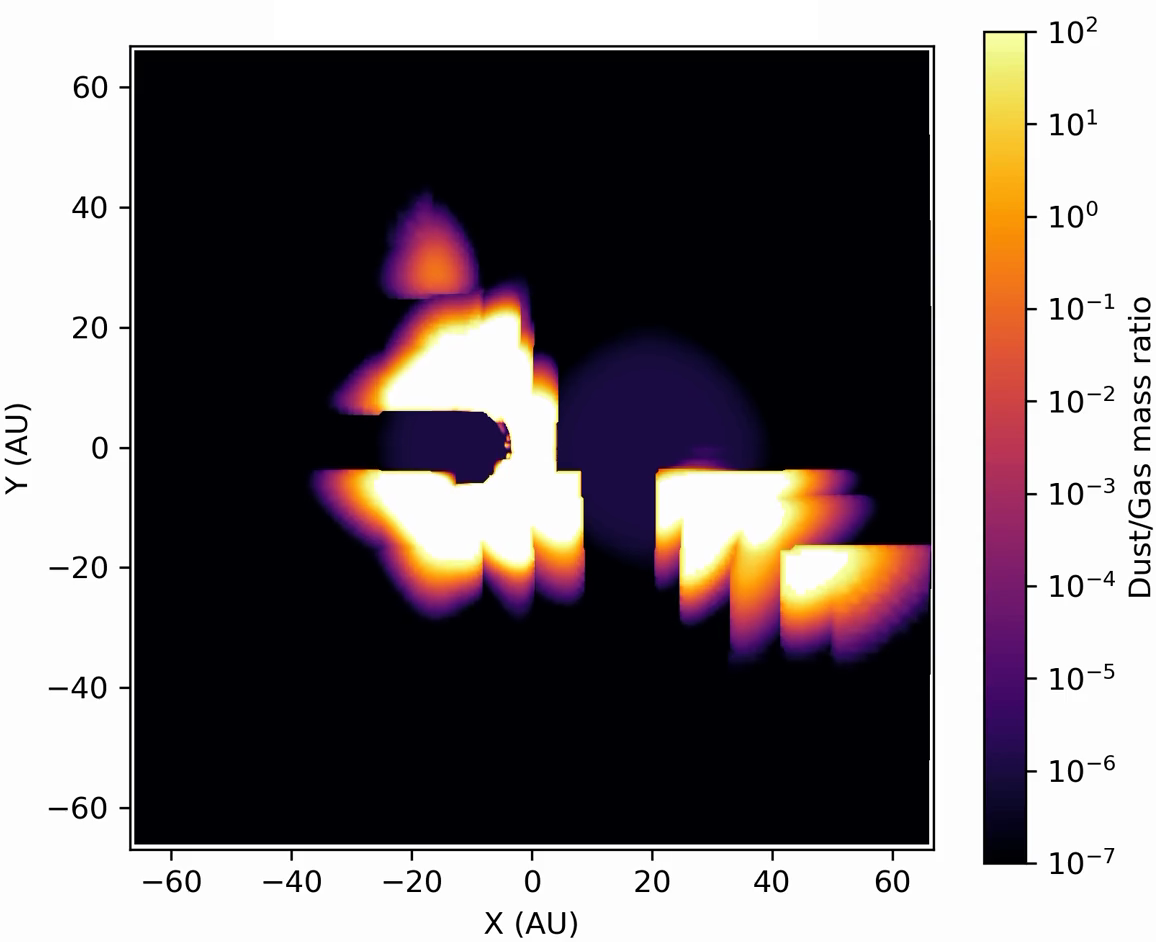
\includegraphics[width=4in]{assets/refinement/breakdown.png}
  \caption[AMR breakdown in \athena]{An example of scalar conservation breakdown in \athena. Continuity is not preserved for scalars between block interfaces and levels, resulting in incorrect behaviour, such as there being more dust than gas within the simulation.}
  \label{fig:amrbreakdown}
\end{figure}

SMR is a significantly simpler method of refining cells, where a region is defined when initialising the simulation which is refined to a higher level.
The code will then progressively de-refine meshblocks beyond this region until the coarsest level is reached.
This method is much less flexible, and is less efficient, but is still useful for simulations where a small region requires a higher spatial resolution at all times. 
In the case of CWB systems this is a reasonably good approximation, as the region around the orbit of the stars can be refined to a higher resolution, while progressively de-refining further out from the barycentre (Fig. \ref{fig:smr-example}).
For the \SI{1000}{AU} simulation requiring \SI{1.07e12} cells, na\"ively refining a region around 1.5 times the orbital separation from the barycentre with 7 refinement levels resulted in a reduction to \num{1.55e6} cells, a 6 order of magnitude reduction in cell count and memory usage.
As such, SMR was used throughout the course of our simulations, as a fix was not available for AMR from the \athena{} developers before publication.

\begin{figure}[ht]
  \centering
  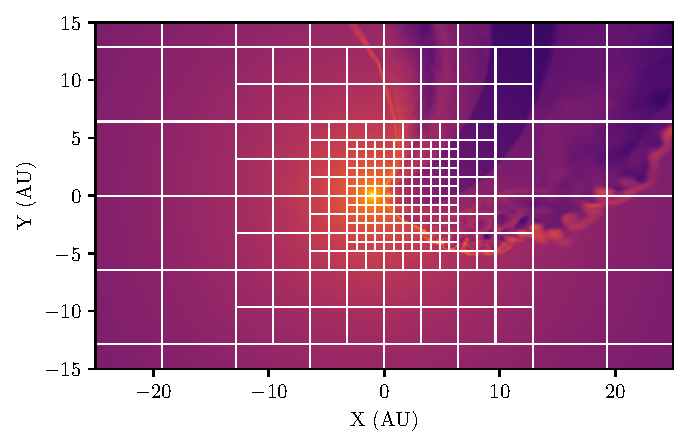
\includegraphics{assets/refinement/wr140/gridref.pdf}
  \caption[Static mesh refinement in \athena]{An example of SMR usage in \athena. A simulation of WR140 was generated with a bounding box around the orbit of the stars at periastron. Within this bounding box the simulation is refined 4 numerical levels deeper than the coarse resolution, and re-refines with distance from the box. The overlaid grid represents individual meshblocks with a resolution of $40\times 40 \times 10$ cells.}
  \label{fig:smr-example}
\end{figure}

\section{Simulating CWB systems}

% Recap why CWB simulations are so complex
As stated in an earlier section, a numerical simulation is only as accurate as its assumptions and input data.
% How is this performed, processes involved in mapping wind on stars, orbits, how these are performed in the context of \athena{} or numsim in general
Our goals for the simulation of dust producing CWB systems throughout this project are as follows:

\begin{itemize}
  \item Two stars are produced and orbit each other with eccentricity $e$ and period $P$ based on star masses $m\rms{WR}$ and $m\rms{OB}$.
  \item The stars should produce a user-defined outflow of wind with mass loss rate $\mdot$ and terminal velocity $\vinf$.
  \item The outflowing wind must be of a pre-defined metallicity, and cool through radiative processes such as forbidden lines, recombination and resonance line emission.
  \item Dust should be able to condense in dense, cool regions.
  \item The resultant dust grains should be able to grow and shrink in accordance with grain growth and grain destruction mechanisms.
  \item The dust should also be able to cool through collisional excitation and subsequent radiative emission.
\end{itemize}

\noindent
As well as the following goals and targets for the model itself:

\begin{itemize}
  \item All radiative processes should be accurate, but not make up a significant fraction of the overall processing time of a cell.
  \item The dust model should be highly modular, and capable of implementing new growth and destruction mechanisms in the future.
  \item The model should be reliable and stable if presented with sensible initial conditions.
  \item Code should be well documented and easy to understand in order to streamline future work from other researchers.
\end{itemize}

\noindent
These goals were achieved, and improvements to the current model have been considered for future implementation.
Initially a multi-fluid model for dust was considered, but could not be implemented in the remaining time in this project.
For future research this would improve accuracy significantly, for a variety of reasons that will be discussed.
In this section we will discuss how the systems are simulated, as well as the assumptions made and specific optimisations made in order to accomplish this task.

\subsection{Assumptions}
\label{sec:simassumptions}

There are a number of assumptions imposed for both the stellar winds and dust within the simulation.
% Short subsection covering assumptions used in this project
Wind self-gravity and gravitational attraction of the wind is neglected.
The outflow velocity of the stars is assumed to be on the order of the system escape velocity, $v\rms{esc}$.
% Wind mapping, lack of radiative line driving
Another assumption is that the outflow from each star is rapidly accelerated to the stars wind terminal velocity, $v^\infty$.
This negates the need for simulating radiative line driving effects on the stellar wind, or calculating the CAK parameters for each wind, however this can result in over-estimation of the wind collision velocity if the wind momentum is sufficiently imbalanced, and the apex of the WCR is close to the secondary star.
If the wind velocity is sufficiently reduced this can effect the structure of the wind collision region, as the wind momentum ratio and cooling parameter will be changed.
Additional factors such as sudden radiative braking can also effect the primary star, where in the case of an extremely unbalanced wind, the primary stellar wind can become rapidly decelerated as it approaches the secondary star and its radiative flux is more influential than the driving force of the parent star \parencite{gayley_sudden_1997}.
This should be considered when analysing the results of each simulation, and understanding how the secondary wind velocity can effect the cooling and dust production rate of the WCR.
% Radiation processes
It is also assumed that all energy radiated leaves the simulation, with no subsequent re-adsorption.
This assumption is valid in the case of mid and far-IR radiation, which is the predominant radiation method in the cool, dense post-shock region.
Whilst re-adsorption and subsequent re-emission would significantly increase the complexity of the simulation, as the effects of radiative transfer would have to be calculated.

% Short coverage on dust model, this is explained further in a alter section
Finally, number of assumptions are made for the dust model.
We assume that the number density of the dust grains is constant, such that the net amount of grains being shattered and grains being agglomerated is zero.
As gas-grain sputtering and coagulation are significantly more common processes and do not change the number density, this is a reasonable assumption considering the dust evolution mechanisms currently implemented and the limitations of an advected scalar model.
We assume that grain growth occurs below \SI{14000}{K}, which is below the sublimation temperature of carbon dust grains.
We also assume grain growth due to grain-gas accretion is approximately 10\% efficient, which is a conservative estimate for grain growth, and could be as high as 100\% in the case of charged dust grains \parencite[Ch.~9]{spitzerPhysicalProcessesInterstellar2008}.

\subsection{Stars, wind propagation \& refinement}

% Orbits
Stars are implemented as point masses, with their orbital positions and velocities governed by Keplerian dynamics.
A solver for the orbital motion is included, and calculates the positions of the stars relative to a Barycenter at simulation position $(0,0,0)$ at every timestep.
The orbital method is 2 dimensional, with both stars at $z=0$ and with no $z$ axis orbital motion.
The solver includes a Newton-Raphson approximation method for improved accuracy.
% Why not gravitational interaction?
As there are only two gravitationally interacting bodies in the system, it was deemed unnecessary to implement a more complex n-body gravitational system to model the dynamics of the stars.
Additionally, calculating the radial velocity at the start of the simulation would be required, all of which is not needed in the case of a Keplerian orbit simulation.
As the orbital path of the system is already known, this also allowed the use of a ``phase offset'' to change the starting point of each simulation, such as in the case of the WR140 simulation, which begins at $\phi = 0.95$.

% Wind propagation
With the assumption that winds are rapidly accelerated to $v^\infty$, propagating stellar winds through a simulation has been drastically simplified.
% Wind remapping
In the simulation, the conserved variables inside a small spherical region 6 fine cells in radius are modified in order to inherent the parameters of a stellar outflow, with a mass loss rate of $\dot{\text{M}}$ and a wind velocity of $v_\infty$ radially outwards from the star.
The conserved variables, correspond to:

\begin{subequations}
  \begin{align}
    \rho_R &= \frac{\dot{\text{M}}}{4 \pi r^2 v_\infty}, \\
    P_R    &= \rho_R v_\infty^*, \\
    E_R    &= \frac{P_R}{\gamma - 1} + \frac{1}{2} \rho_R v_\infty^2,
  \end{align}
\end{subequations}

\noindent
where $r$ is the radial distance from the star, $P_R$ is the cell pressure, and $\gamma$ is the ratio of specific heats, typically $5/3$.
Whilst this method is very fast and effective, it requires the remap region to remain completely undisturbed, if the WCR impinges upon the remap region this will result in significant physical inaccuracy.
In order to mitigate this, it was found that there should be $75-120$ fine cells separating the stars, for a system with $\eta\sim 0.01$.
For systems with a WCR closer to the secondary star the number of cells should be significantly increased.
 
% How refinement is performed 
Throughout this thesis SMR is used to increase the effective resolution of simulations, a box around the CWB orbit is refined to the highest level defined in the simulations input file, \athena{} de-refines the cells gradually around this box until the simulation is at its coarsest resolution.

\subsection{Cooling in numerical simulations}

% Brief recamp on radiative cooling processes, compare with physical section, why they are important in the context of our work
As discussed in section \ref{sec:wcrcooling}, there are many cooling processes that need to be considered when simulating a complex system such as a CWB.
Sufficient cooling is in fact, essential to this dust formation process.
Gas temperature in the immediate post-shock region can exceed $10^8\, \si{\kelvin}$, far beyond the temperatures required to adequately form dust, as any nascent grains would quickly be shattered by thermal processes.
There is sufficient evidence to suggest that significant, rapid temperature loss occurs in the post-shock regime, the high metallicity of the WC wind and high number density of atoms and ions makes it the ideal region for rapid cooling due to radiative processes.

% Why even include cooling
Another boundary to dust formation due to an insufficiently radiative post-shock flow is a lack of sufficient downstream density.
In the case of strong, adiabatic shocks, constraints are set on the downstream gas parameters of the system, such that:

\begin{subequations}
  \begin{align}
    u_b    & = \frac{1}{4} u_a , \\
    \rho_b & = 4 \rho_a , \\ 
    P_b    & = \frac{3}{4} \rho_a u_a^2 ,
  \end{align}
\end{subequations}

\noindent
where $a$ is the upstream side and $b$ is the downstream, post-shock side.
As the gas density can only be a factor of 4 larger than the post-shock flow, the post shock density (even if it were at  temperatures suitable for dust formation) is insufficiently dense for sufficient dust production.
However, in a radiative shock behaving isothermally (where the temperature change, $\Delta T$ throughout the entire lifespan of the fluid is equal to zero), the final density, $\rho_f$ can be approximated to:

\begin{equation}
  \rho_f \approx \gamma M_a^2 \rho_a,
\end{equation}

\noindent
where $M_a$ is the pre-shock mach number.
For a shock with an initial sound speed of $M_a = 100$ the final density can exceed the pre-shock density by a factor of $10^4$!

% Complexities, conservation, that kind of thing

Performing radiative cooling within a numerical simulation is computationally difficult, and trade-offs between accuracy and performance must be considered at every step of designing the simulation, as every single cell must undergo cooling.
For this project, the final cooling can be out by a few percent at worst, but is fast enough to run the simulations in a reasonable amount of time without excessive memory requirements.
In order to simplify the radiation calculations, radiation does not re-interact with the simulation, instead it is completely removed from the simulation.
Due to this, scattering, re-adsorption and radiative transfer are not simulated at all.\footnote{If these are considered, your programme is now a ray-tracing programme as well as a hydrodynamical code, which is its own, even more complicated field.}.
Other methods of reducing computational cost and optimising the code are used in this project, and will be described in detail in this section.

\subsection{Plasma cooling}

% This isn't a section on the radiative processeses themselves, but more to do with how plasma cooling is simulated 
Cooling due to radiative emission of gas and plasma is a very complex topic, and has to factor in multiple mechanisms of emission, which are heavily dependent on the elemental abundance of a wind.
Cooling codes such as MEKAL are used to calculate the emissivity, $\Lambda$, of a wind given the current temperature, abundance and density
\parencite{meweCalculatedXradiationOptically1985,meweCalculatedXradiationOptically1986}.
However, these codes are somewhat computationally complex, and are therefore difficult to solve for every cell at every timestep, and as such, is abstracted by use of a lookup table.
% Use of a lookup table
This lookup table is pre-calculated and loaded into the simulation at runtime and are generated by combining a series of lookup tables generated for pure flows of elements, and combined based on the abundance of the element within the stellar wind.
As such, both stars have their own unique lookup table.
A typical lookup table in this project utilises logarithmically spaced temperature bins from $10^4\,\si{\kelvin}$ to $10^9\,\si{\kelvin}$, with 100 bins in total, if the calculated temperature is between bins a linear interpolation step is used to improve the accuracy of the emissivity solution.
In order to calculate the energy loss due to emission from atoms and ions within a cell, the following formulae is used:

\begin{equation}
  \mathcal{L}\rms{g} = \left(\frac{\rho}{m_H}\right)^2 \Lambda\rms{g} (T) ,
\end{equation}

\noindent
where $\Lambda\rms{g}(T)$ is the normalised emissivity at the cell temperature, T.
This solution is orders of magnitude faster than performing an emissivity calculation in every cell, and is essential to performing fast hydrodynamical simulations with plasma radiative cooling.

% Mean molecular mass


% Improvements to accuracy of lookup table, linear search
Other optimisations relied on replacing a na\"ive linear search with an indexing method that relied on the logarithmic spacing of the temperature bins, instead of performing a search the index, $n$, of the emissivity value stored in an array can be calculated using the formulae

\begin{equation}
    n = \left \lfloor \frac{\log(T) - \log(T)_\text{min}}{\delta \log (T)} \right \rfloor ,
\end{equation}

\noindent
where $\log(T)$ is the log of the cell temperature, $\log (T)_\text{min}$ is the minimum log temperature in the lookup table and $\delta \log (T)$ is the log spacing of the temperature bins. 
This speed-up is fairly significant as the average search performance changes from $\mathcal{O}(n)$ to $\mathcal{O}(1)$ time, a marked improvement over even a binary search, which would resolve in an average of $\mathcal{O}(\log n)$ time.
In the case of a 100 bin array this is only a minor speed-up, but with the sheer number of calculations being performed, any optimisation to a function used multiple times per cell can significantly improve performance.
In the case of larger, or multi-parameter lookup tables this method would only improve in performance, and is a good example of general optimisation in a numerics programme.

% Method of integration chosen
In order to integrate the energy loss rate to determine the exact amount of energy lost within a timestep, an integration method needs to be chosen, for this project, a fast, first-order Euler method with multiple sub-steps was chosen. Whilst this method is not particularly accurate or robust, it was found to be fast, and the adaptive sub-step method was found to calculate a reasonably accurate approximation of a cells change in temperature in a very small amount of time. This sub-step method is elaborated on in section \ref{sec:cooling-implementation}.

\subsubsection{Other calculation methods}

% Why is the estimated method used? see: dust cooling, multiple winds
Other methods of refining the emissivity value were also considered, such as fitting a local curve to the data or using a spline-based interpolation step instead of a linear step, however these were only marginally more accurate, at a significantly increased calculation time. 
An exact cooling method was also considered, which was found to be significantly more performant, but had a series of limitations that prevented it from being used in the codebase at this time.
% Explanation of method, complex bit
This exact cooling method, described by \textcite{townsendExactIntegrationScheme2009}, introduces a temporal evolution function (TEF), $Y(T)$, into the solution, which describes a measure of the total time required to cool from an arbitrary temperature to $T$.
This function, as well as its inverse, need to be calculated prior to the start of simulation, but do not have to be calculated for every cell and timestep.
While solving the TEF for the cell temperature takes approximately the same amount of time as a single first order Euler method integration, an \emph{exact} calculation of the post-step temperature is found.
% Why would this be good
This scheme is one of the rare example of a numerical method that is both accurate \emph{and} fast, taking approximately the same time as a second order explicit method overall, whilst also being perfectly accurate even in highly radiative hypersonic flows.
% Why did we not use it
Unfortunately this method has a number of limitations that precluded its usage in this project.
First, this method would not have been able to accurately model mixed wind situations, hampering its usage cooling winds with drastically different abundances.
Second, and most importantly, dust cooling could not have been modelled with this single parameter TEF method, which would have required using a two stage cooling method.
As the gas temperature would not be synchronised between stages, this would have resulted in a highly inaccurate cooling solution, obviating the advantages of the exact cooling method.

\subsection{Dust cooling}
\label{sec:dustcoolingmodel}

% Discuss dust cooling in brief, link to section in background, touch on lambda being dependent on 3 rather than 1 value

We have previously discussed the underlying physics of dust cooling in Section \ref{sec:dustcooling-background}.
In particular, we discussed that photon emission from dust is primarily due to grain heating through collisional excitation, which in turn causes the heated grain to emit radiation in a method approximating a black body.
This produces an approximately continuous spectra, dependent primarily on the grain size, grain temperature and number density of particles in the surrounding fluid.

Gas and plasma emissivity for a wind of a specific elemental composition is only dependent on temperature, $\Lambda\rms{g}(T)$, with a corresponding energy loss rate of $\mathcal{L}\rms{g} (n\rms{H},T) = n\rms{H} \Lambda\rms{g}(T)$. 
This is convenient for the sake of calculating gas cooling, as the calculation of the emissivities of thousands of emission lines and multiple radiative mechanisms across a temperature domain from $10^4\, \si{K}$ to $10^9\,\si{K}$ would be exceedingly computationally demanding.
Instead, we can use a lookup table, as described in the previous section.
Unfortunately, while the calculation of emission rate of a dust grain is simpler and does not depend on many discrete calculations, it is dependent on more parameters, which can change per cell.
We find that the energy loss rate due to dust is calculated by the formulae:

\begin{equation}
  \mathcal{L}\rms{d} = n\rms{w} n\rms{d} \Lambda\rms{d}(\rho\rms{w},a,T) ,
\end{equation}

\noindent
where $r\rms{w}$ is the wind number density and $\rho\rms{w}$ is the wind density. 
Therefore, in order to calculate energy loss due to dust emission, we must either build a far more complex lookup table, or determine methods of calculating energy loss quickly.
In this section we will discuss the pros and cons of both methods, and discuss our final methodology used in this project.

% Why so significant?

When debating whether or not to include a feature in a numerical simulation, we must weigh up the computational cost versus necessity of inclusion.
In the immediate post-shock environment we find that the cooling rate due to dust is significantly higher than the cooling due to gas and plasma ($\mathcal{L}\rms{g} < \mathcal{L}\rms{d}$) by approximately a factor of five (Fig. \ref{fig:postshockcoolcomparison-chapter3}).
Dust cooling therefore can play an important role in the initial cooling of the post-shock cooling, resulting in faster cooling to temperatures suitable for grain growth.
As such, dust cooling should ideally by included in these simulations.

\begin{figure}[h]
  \centering
  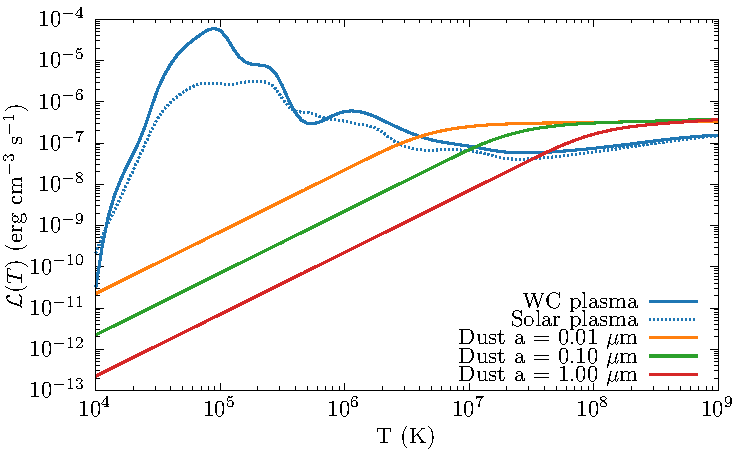
\includegraphics{assets/dust-plasma-cooling-comparison/cooling-comparison-forpaper2.pdf}
  \caption[Comparison of dust and plasma cooling rates in post-shock environment]{Comparison of energy loss due to plasma \& dust cooling with varying grain sizes in a typical post-shock flow, where $\rho_g = 10^{-16} \, \si{\gram\per\centi\metre\cubed}$ and a dust-to-gas mass ratio of $10^{-4}$. Whilst less influential at lower temperatures, dust cooling can aid cooling in the immediate post-shock environment.}
  \label{fig:postshockcoolcomparison-chapter3}
\end{figure}

% Underlying calculation, in depth, 

Throughout this project, we utilise the \textcite{dwek_infrared_1981} prescription for dust radiation emission.
In the case of a dust grain of radius $a$ flowing through a pure elemental gas with an atomic mass $m$ and a number density $n$, 

\begin{equation}
  \begin{split}
    H & = \left(\frac{32}{\pi m}\right)^{1/2} n\pi a^2 (k_B T)^{3/2} h(a,T) \\
    & = \num{1.26e-19} \frac{n}{A^{1/2}} a^2 (\si{\micro\metre}) T^{3/2} h(a,T) \, \si{\erg\per\second}
  \end{split}
\end{equation}

\noindent
where $A$ is the atomic mass of the gas in AMU and $h(a,T)$ is the effective grain heating factor.
This last parameter, also referred to as the grain ``transparency'', is the 

% Effective heating for atoms

% Creati

This critical energy varies depending on the atom and the grain size, and was calculated by \textcite{dwek_infrared_1981} to be 
$23 a^{2/3} (\si{\micro\metre})$ for electrons,
$133a(\si{\micro\metre})$ for hydrogen,
$222a(\si{\micro\metre})$ for helium,
and $665\times a(\si{\micro\metre})$ for metals.
The grain transparency can then be calculated using the formulae:

\begin{equation}
  h(a,T) = 1 - \left(1 + \frac{E^*}{2k\rms{B} T}\right) e^{E^*/k\rms{B}T} .
\end{equation}
% Effective heating for electrons
\noindent
Calculating the grain heating factor for electrons is markedly more difficult, in the uncharged case we find that

\begin{equation}
  \label{eq:heintegral}
  h\rms{e}(a,T) = 1 - \frac{e^{x^*}}{2} \int^\infty_0 \mathcal{K}(x^*,z) dz 
\end{equation}

\noindent
where

\begin{equation}
  \mathcal{K}(x^*,z) = (z + x^*) \left[ (z + x^*)^{3/2} - {x^*}^{3/2} \right]^{2/3} e^{-z} , 
\end{equation}

\noindent
where $x^* = E^* / k\rms{B} T$ and $z$ is an arbitrary value.

% Difficulty of calculating h_e, expand on in integration method subsubsection
Performing an indefinite integral inside of a hydrodynamical code is not ideal, and must be either constrained or simplified in such a way where it can be made performant.
Additionally, electron-grain heating cannot be discounted, as it typically outweighs atom-grain heating more than 2 orders of magnitude (see Section \ref{sec:dustcooling-background}, Fig. \ref{fig:collisionalheatingcomparison}).
% Other difficulty of electrons, free ions
Another factor in determining the contribution due to free electrons was determining the free electron number density, which can vary significantly with temperature in a highly metallic wind.

We trialled two methods involving solving the integral, before settling on using an approximation described in \textcite{dwek_infrared_1981}.

% Difficulties in dust cooling integral, faster method of doing this
\subsubsection{Integration Method}

\begin{figure}[ht]
  \centering
  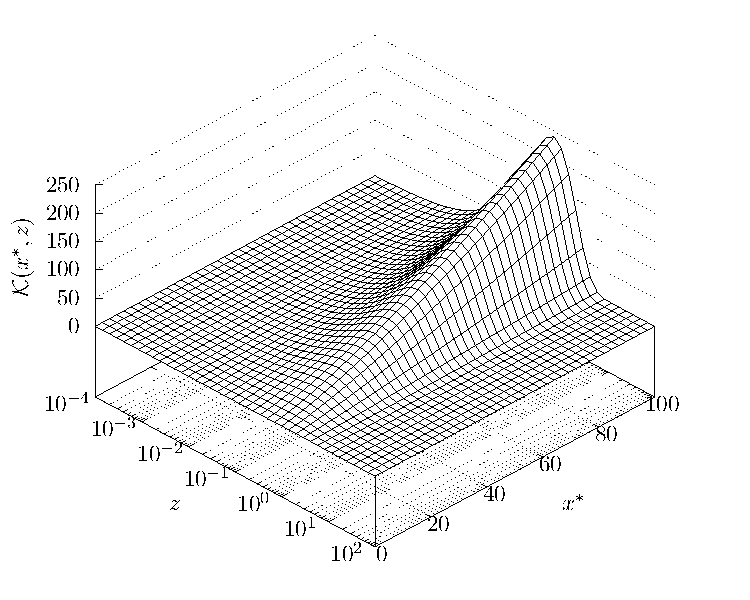
\includegraphics{assets/integral/func_xe_3d.pdf}
  \caption[3D plot of $\mathcal{K}(x^*,z)$]{Surface plot of $\mathcal{K}(x^*,z)$, for a given $x^*$ we can see that $\mathcal{K} \rightarrow 0$ before $z = 100$, suggesting that the integral can be constrained from $z=10^{-3}$ to $z=10^2$.}
  \label{fig:constrainplot3d}
\end{figure}

\begin{figure}[ht]
  \centering
  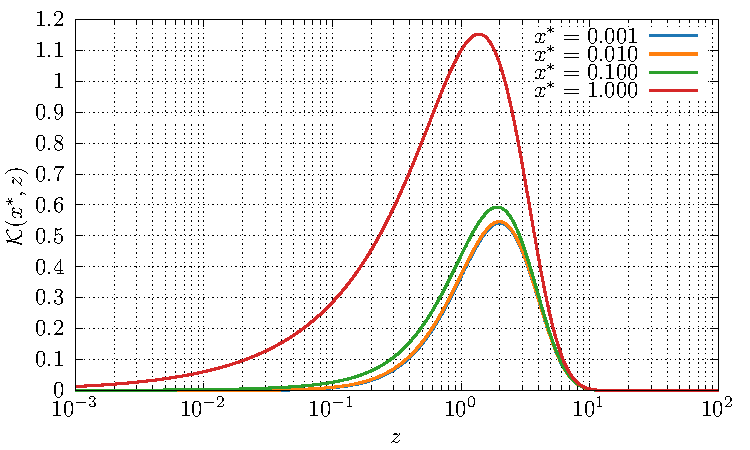
\includegraphics{assets/integral/func_xe_plot.pdf}
  \caption[Plot of $\mathcal{K}(x^*,z)$ for discrete values of $z$]{Plot of $\mathcal{K}(x^*,z)$ with values of $z$ between 0.001 and 1, we see that the plot can moderately well constrained between $z=10^{-3}$ and $z=10^2$.}
  \label{fig:constrainplot2d}
\end{figure}

The first, and most na\"ive method of determining $h_e$ was by calculating an approximation of $h_e$ for each cell at each cooling step.
The integral described in Eq. \ref{eq:heintegral} can be constrained and calculated using a definite integral method such as the trapezium rule.
It was determined that the equation peaks at $z \approx 1$ in all cases, and quickly tapers off to $0$ before $z=100$ (Fig. \ref{fig:constrainplot3d} \& \ref{fig:constrainplot2d}).
The integral was constrained such that

\begin{equation}
  h_e = 1 - \frac{e^{x^*}}{2} \int^{10^2}_{10^{-2}} \mathcal{K}(x^*,z) dz,
\end{equation}

\noindent
and solved through the trapezium method with logarithmically spaced bins.
While this integral can be constrained in such a manner, it was found that a large number of bins was required to solve the equation correctly (Fig. \ref{fig:he-accuracy-bins}).
It was found that 400 bins was the minimum amount required to reliably calculate $h_e$, which would result in the integral taking approximately 90\% of the overall execution time of the cooling step.
Values below 400 bins would result in negative values for $h\rms{e}$, which would render the simulation completely unphysical.
Subtle improvements to performance could be made by forcing $h
rms{e} = 1.0$ for temperatures below $10^6 \, \si{K}$, but this was found to still be comparatively slow.
A more complex integration method would not improve performance at this point, instead, other methods were considered.

\begin{figure}[ht]
  \centering
  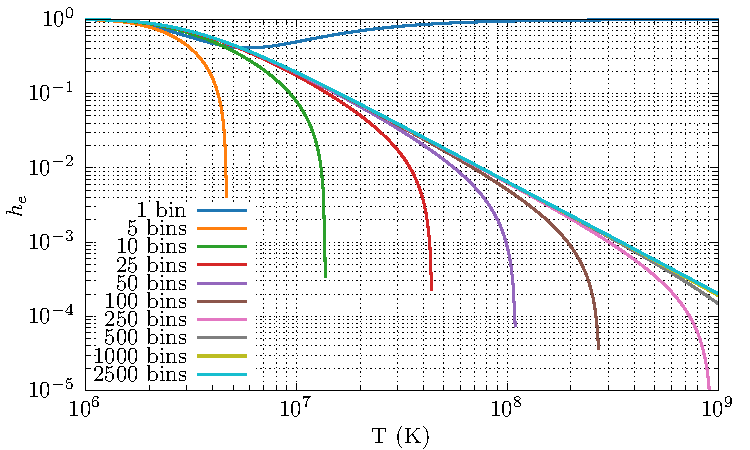
\includegraphics{assets/he_accuracy/he_acc.pdf}
  \caption[$h_e$ integration accuracy comparison]{Comparison of $h_e$ as a function of temperature for dust grains with a radius of 0.005 \si{\micro\metre}, $h_e$ is calculated via the trapezium rule with a varying number of bins, bin counts below 400 bins result in wildly inaccurate or in some case negative values for $h_e$, while beyond 400 bins the result is accurate and converges slowly.}
  \label{fig:he-accuracy-bins}
\end{figure}

\subsubsection{Lookup table}

Another method considered was the use of a multidimensional lookup table, containing values for $\Lambda\rms{d}$ for specific values of $\rho\rms{g}$, $T$ and $a$.
A moderately sized array of $101\times 101 \times 101$ elements was used, with a total of 1030301 possible values of $\Lambda\rms{d}$, spaced logarithmically.
The values for $\Lambda$ were generated from the integral method of solving Eq. \ref{eq:heintegral} using a \num{10000} bin integration with a parameter space described in Table \ref{tab:lookupparams}.

\begin{table}[ht]
  \centering
  \begin{tabular}{llll}
  \hline
  Parameter & Min & Max & Bins \\ \hline
  $\rho\rms{g}$ & \SI{1e-25}{g.cm^{-3}}   & \SI{1e-10}{g.cm^{-3}}  & 101 \\
  $T$           & \SI{1e4}{K}               & \SI{1e9}{K}            & 101 \\ 
  $a$           & \SI{1e-3}{\micro\metre} & \SI{1e2}{\micro\metre} & 101 \\
  \hline
  \end{tabular}
  \caption{Parameter space of $\Lambda\rms{d}$ 3-parameter lookup table.}
  \label{tab:lookupparams}
\end{table}

Similarly to the 1D lookup table used for gas cooling, for each parameter, $P$, we determine the closest value smaller than ($P\rms{l}$) and greater than ($P\rms{u}$) the actual value.
This is then used to calculate an offset, $P\rms{d}$:

\begin{equation}
  P\rms{d}=\frac{P-P\rms{l}}{P\rms{u}-P\rms{l}} , 
\end{equation}

\noindent
these offsets are then used to perform a trilinear interpolation to calculate $\Lambda\rms{d}$ from the lookup table, through the equation:

\begin{equation}
  \begin{split}
    \Lambda\rms{ll} &=\Lambda\rms{lll}\left(1-\rho\rms{d}\right)+\Lambda\rms{ull} \rho\rms{d}, \\
    \Lambda\rms{lu} &=\Lambda\rms{llu}\left(1-\rho\rms{d}\right)+\Lambda\rms{ulu} \rho\rms{d}, \\
    \Lambda\rms{ul} &=\Lambda\rms{lul}\left(1-\rho\rms{d}\right)+\Lambda\rms{uul} \rho\rms{d}, \\
    \Lambda\rms{uu} &=\Lambda\rms{luu}\left(1-\rho\rms{d}\right)+\Lambda\rms{uuu} \rho\rms{d}, \\
    \Lambda\rms{l} &=\Lambda\rms{ll}\left(1-a\rms{d}\right)+\Lambda\rms{ul} a\rms{d}, \\
    \Lambda\rms{u} &=\Lambda\rms{lu}\left(1-a\rms{d}\right)+\Lambda\rms{uu} a\rms{d}, \\
    \Lambda\rms{d} &=\Lambda\rms{l}\left(1-T\rms{d}\right)+\Lambda\rms{u} T.
  \end{split}
\end{equation}

\noindent
This method is markedly faster, and can be improved if multiple cooling sub-steps are performed.
As the same offset, upper and lower values for $\rho\rms{g}$ and $a$ , as they are invariant over a time-step in any given cell.
Further improvements through handwritten unrolled loops and optimisation for SIMD were performed to improve performance by a factor of two.
This final bilinear+linear method improves performance from the integral method by approximately \num{1800}\%, and can scale well within a numerical simulation (Fig. \ref{fig:dust-opt-speedup}).

\begin{figure}[ht]
  \centering
  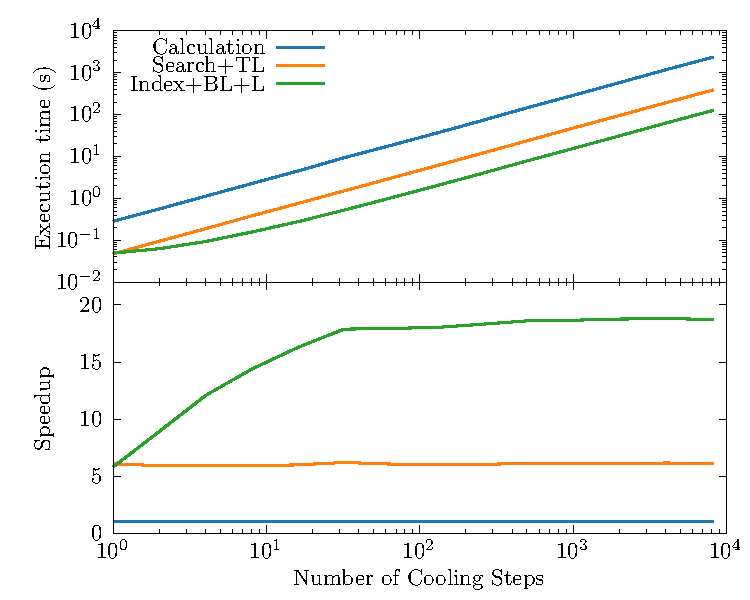
\includegraphics{assets/lambda-dust-speedup/lambda-dust-speedup.pdf}
  \caption[Dust lookup table methods comparison]{Comparison of execution time and speedup for lookup table methods.}
  \label{fig:dust-opt-speedup}
\end{figure}

\subsubsection{\textcite{dwek_infrared_1981} approximation}

\textcite{dwek_infrared_1981} provide a series of equations to estimate $h\rms{e}$ based on the value of $x^*$:

\begin{equation}
  \begin{alignedat}{3}
    h_e(x^*) & = 1 ,                && ~~ x^* > 4.5, \\
    & = 0.37{x^*}^{0.62} , && ~~ x^* > 1.5 , \\
    & = 0.27{x^*}^{1.50} , && ~~ \text{otherwise.}
  \end{alignedat} \label{eq:electrontransparencyestimate}
\end{equation}

\noindent
This method is less accurate, especially between cases, but is multiple orders of magnitude faster.
We find this estimate is at worst divergent from the integral method by $8\%$, and closely matches the results from the integral method (Fig. \ref{fig:lambda-comp-int-vs-est}).
After some optimisation, the resultant estimate was found to be approximately \num{25000}\% faster than the integral method, meaning the electron contribution to dust cooling has a negligible impact on processing time of a single time-step.
Table \ref{tab:electron-speedup} shows the results of benchmarking attempts on all of the methods tested, as we can see, the approximation method is by far the fastest method, with an acceptable worst-case deviation from the integral method result.
Because of this, it was decided that the approximation method would be used.

\begin{figure}[ht]
  \centering
  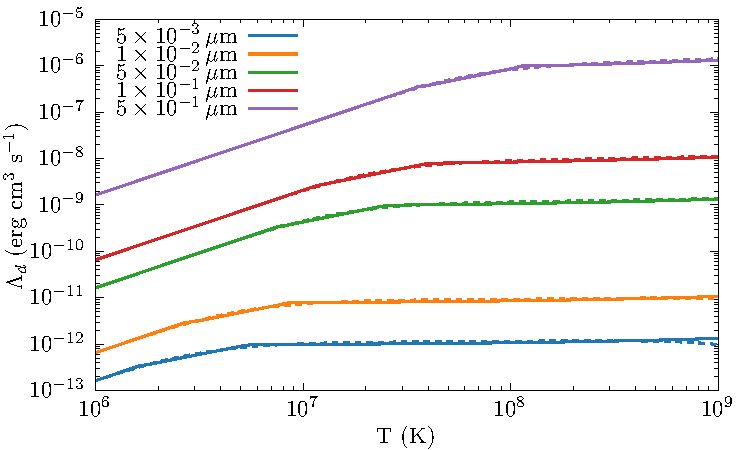
\includegraphics{assets/grain-transparency/lambda-comp.pdf}
  \caption[Electron transparency method accuracy - $\Lambda_d$]{$\Lambda_d$ as a function of temperature for various grain sizes and solar abundances. Solid lines represent calculations from the \textcite{dwek_infrared_1981} estimation, dashed lines represent the integral method. The estimation method is extremely close to the integral value aside from at the highest temperatures.}
  \label{fig:lambda-comp-int-vs-est}
\end{figure}

\begin{table}[ht]
  \centering
  \begin{tabular}{lllll}
    \hline
    Method & t(s) & Iter/s & Speedup & Worst result \\ \hline
    400-bin integration & 36.03 & 35,526 & - & 0\% \\
    Trilinear & 6.016 & 212,751 & 599\% & 0.3\% \\
    Bilinear + linear & 1.999 & 640,447 & 1,803\% & 0.3\% \\
    Approximation & 0.147 & 8,693,171 & 24,510\% & 8\% \\ \hline
  \end{tabular}
  \caption[Dust cooling calculation comparison]{Comparison of methods explored for estimating $\Lambda_d(\rho,a,T)$ in cooling code, $10^4$ initial values were chosen and 128 cooling sub-steps were performed, benchmark code was compiled and run using \texttt{GCC 10.3.0} with the \texttt{-O3} optimisation set on an Intel i7-7700HQ processor with a maximum clock speed of \SI{3.8}{\giga\hertz}.}
  \label{tab:electron-speedup}
\end{table}

\subsubsection{Calculating $n\rms{e}$}

Initially, a solar abundance approximation of the electron number density, $n\rms{e}$, was used, where $n\rms{e} = 1.32 n\rms{H}$, where $n\rms{H}$ is the expected number density in a pure hydrogen flow ($n\rms{H} = \rho\rms{g} / m\rms{H}$).
This can vary as much as a factor of 3 in the case of a WC wind, and vary significantly from $10^4 \, \si{K} \rightarrow 10^7 \, \si{K}$ as the wind becomes increasingly ionised.
A logarithmically spaced lookup table similar to the plasma cooling curve was used, containing the electron-to-ion ratio between $10^4$ and $10^9$ kelvin for both winds (Fig. \ref{fig:electron-curve-no-elements}). 
This method was found to be comparatively fast, as the index method and calculation of the ion number density are computational trivial.

\begin{figure}[h]
  \centering
  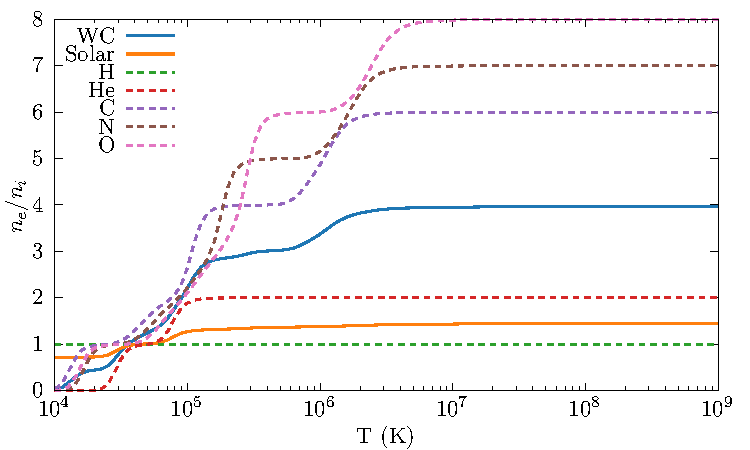
\includegraphics{assets/ionisation-fraction/ionisation-fraction.pdf}
  \caption[OB and WR electron-ion ratios]{A comparison of the electron-ion ratio in both winds as a function of temperature. Also shown are the electron-to-ion ratios for the individual elements.}
  \label{fig:electron-curve-no-elements}
\end{figure}

\subsection{Model implementation}
\label{sec:cooling-implementation}

In order to simulate energy loss due to radiation in \athena{}, the conserved variable array is adjusted to remove energy from a specific cell, this is analogous to energy being removed from the system due to radiative processes in an optically thin gas.
% Flesh out cooling problem in general
Radiative processes are part of a source function that is performed for every mesh block.
The cooling routine within the source function iterates through all cells within the meshblock, calculating radiative energy loss for each cell.
% Lookup table method recap + how it is applied
Within the loop, the cell parameters are loaded from the conserved variables array, and additional gas and dust parameters are calculated from these conserved variables.
in particular the mean molecular mass of a cell is calculated with the formulae:

\begin{equation}
  \mu = C\mu_{WR} + (1-C) \mu_{OB}, \label{eq:windaveraging}
\end{equation}

\noindent
where $\mu_{WR}$ and $\mu_{OB}$ are the mean molecular masses of the winds and $C$ is the wind ``colour'' scalar, the contribution of each wind to the gas density of the cell.
The temperature is subsequently calculated using the ideal gas law:

\begin{equation}
  T = \frac{P \mu m_H}{\rho k_B}.
\end{equation}

\noindent
At the current temperature, the cooling parameter, $\Lambda\rms{g}(T)$ for each wind is found from the lookup tables, and weighted in a similar manner as equation \ref{eq:windaveraging}. The energy loss due to dust grains is then calculated, with the total energy loss rate per unit volume within the cell defined as:

% \begin{equation}
%   \mathcal{L} = _\text{G} + _\text{D} = \left(\frac{\rho}{m_H}\right)^2 \Lambda_\text{G}(T) + n_\text{D} _\text{grain},
% \end{equation}

\begin{equation}
  \mathcal{L} = \mathcal{L}\rms{g} + \mathcal{L}\rms{d} = \left(\frac{\rho\rms{g}}{m\rms{H}}\right)^2 \Lambda\rms{g} + \left(\frac{\rho\rms{g}}{\mu m\rms{H}}\right) n\rms{d} \Lambda\rms{d}(\rho\rms{g},a,T),
\end{equation}

\noindent
where $\rho\rms{g}$ is the gas density,
$m\rms{H}$ is the mass of a hydrogen atom,
and
$n\rms{d}$ is the dust number density.

% Timestep method, why is this used rather than a single timestep

Performing the exact calculation of $\mathcal{L}$ as described in \textcite{townsendExactIntegrationScheme2009} would only work for gas cooling, and would require significant modification to work with a combination of gas and dust cooling.
Mixed winds are also not supported, and the amount of cooling varies significantly based on the level of metallicity within a system, thus this is significantly less accurate for this use-case.
Adaptive sub-stepping is utilised instead to improve accuracy of a fast Euler integration by increasing the temporal resolution in cases of rapid cooling.
At the end of each sub-step, after $\mathcal{L}$ is calculated, a cooling time is calculated using the formulae:

\begin{equation}
  \tau\rms{cool} = \frac{E_i}{\mathcal{L}} ,
\end{equation}

\noindent
where $E_i$ is the internal energy of the cell.
A fraction of this cooling time is used as a time-step if $\kappa \tau\rms{cool} \leq t\rms{rem}$, where $\kappa$ is a user-defined fraction and $t\rms{rem}$ is the remaining time in the time-step.
This process is repeated until the time-step is completed.
Throughout this project we adopt a value for $\kappa$ of $0.1$.
This method allows for more accurate calculations of cooling in cells with a higher cooling rate, while also being very fast in regions that are not undergoing excessive cooling.
Fig. \ref{fig:cooling-loop-evolution} shows the adaptive sub-stepping routine in operation, at the initial time, the cooling parameter $\Lambda$ is maximised, as such the time-step is significantly lower than when the gas has cooled as is less radiative.
This compares favourably to a single sub-step example, which would cause the simulation to crash due to negative temperatures, and with linearly spaced steps, which either required many more steps or were potentially unstable.

\begin{figure}[ht]
  \centering
  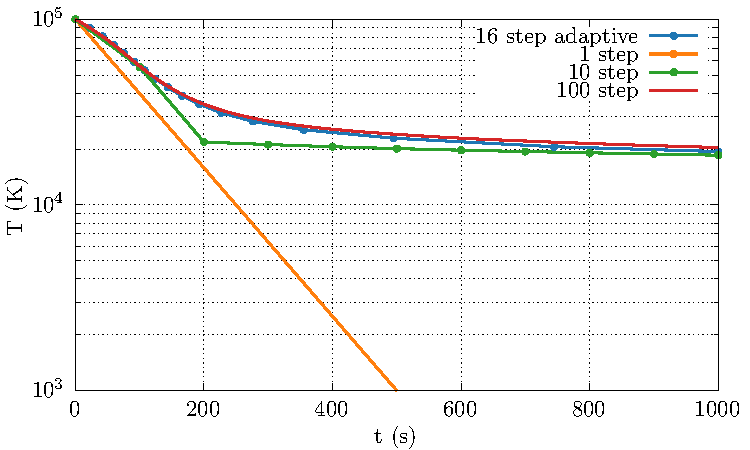
\includegraphics{assets/plasma-cooling-benchmarks/evolution.pdf}
  \caption[Cooling sub-step method evolution comparison]{Comparison of the adaptive timestep method versus linearly spaced sub-steps for a solar abundance flow with a density of $10^{-16}$ \si{\gram\per\centi\metre\cubed} and an initial temperature of $10^5$ \si{\kelvin}. Cooling was artificially limited to prevent negative temperatures, which would have occurred in the case of the 1 sub-step method.}
  \label{fig:cooling-loop-evolution}
\end{figure}

Additional testing with starting temperatures of $10^5 \, \si{K}$, $10^6 \, \si{K}$ and $10^7 \, \si{K}$ and similar parameters to Fig. \ref{fig:cooling-loop-evolution} were used to determine the accuracy of the sub-step method versus the exact integration method proposed in \textcite{townsendExactIntegrationScheme2009}.
$\kappa$ was also varied, in order to determine a suitable value with a reasonable error of no more than $10\%$ at worst. 
Table \ref{tab:cooling-loop-accuracy-comp} shows that $\kappa = 0.1$ produces an error of $6\%$ at worst, while $\kappa = 0.01$ requires an order of magnitude more sub-steps to improve the accuracy to $1\%$.
This is due to the slow convergence time of a first-order integration method such as Euler integration, but this error was deemed acceptable.
At higher temperatures and less intense cooling we find fewer sub-steps are required to calculate $\mathcal{L}$, with much greater accuracy.
A single sub-step took an average of \SI{134}{\nano\second} using the adaptive sub-step method, while the \textcite{townsendExactIntegrationScheme2009} method took \SI{151}{\nano\second}, when conducted on a \SI{3.2}{\giga\hertz} M1 ARM processor with \texttt{O3} optimisation.
The speed benefit of the estimation method is diminished at lower temperatures, but is necessary considering the limitations of the \textcite{townsendExactIntegrationScheme2009} method.
Whilst this is a fairly simplistic method of performing adaptive sub-stepping, it is fast, effective, and not prone to failure.
Improved models in the future could utilise an adaptive RK method, in a similar manner to the numerical integrator in \athena{}, though the implementation attempted had some numerical stability and execution time issues, and would require significant optimisation.

\begin{table}[h]
  \centering
  \begin{tabular}{lllllll}
  \cline{2-7}
   & \multicolumn{2}{l}{$\kappa = 0.1$} & \multicolumn{2}{l}{$\kappa = 0.01$} & \multicolumn{2}{l}{$\kappa = 0.001$} \\ \hline
  $T_i$ & Steps & Error & Steps & Error & Steps & Error \\
  \hline
  $\SI{1e5}{\kelvin}$ & 16 & \num{6.025e-02} & 159 & \num{1.282e-02} & 1585 & \num{7.637e-03} \\
  $\SI{1e6}{\kelvin}$ & 1 & \num{8.233e-04} & 6 & \num{1.012e-04} & 58 & \num{3.359e-05} \\
  $\SI{1e7}{\kelvin}$ & 1 & \num{1.577e-07} & 1 & \num{1.577e-07} & 2 & \num{1.411e-07} \\ \hline
  \end{tabular}
  \caption[Cooling method accuracy comparison]{Accuracy of the adpative sub-step Euler method compared with the \cite{townsendExactIntegrationScheme2009} exact cooling method, with $\kappa = 0.1$ this method is out by $6\%$ at worst in the low-temperature example, while very accurate at higher temperatures with only a single step needed.}
  \label{tab:cooling-loop-accuracy-comp}
\end{table}

\section{The \bidmas{} Advected Scalar Dust Model}
\label{sec:bidmas}

For this thesis, it was decided from the beginning to implement a dust model within a numerical simulation.
This dust model would operate first with advected scalars, before moving on to a more complex multi-fluid model.
Additionally, this model was designed be extensible, implementing grain destruction and accretion mechanisms that were the most influential first.
The Binary Interaction Dust Model with Accretion and Sputtering (\bidmas{})\footnote{Any good thesis (though this one, again, is of debatable quality) has an incredibly laboured acronym!} model is the result of this work, and while in a relatively simple state due to the previously stated time restrictions, is a good first step towards modelling WCd systems.

\subsection{\bidmas{} features}

% Broad featureset
Currently the \bidmas{} model supports grain advection and destruction, as well as the dust cooling model discussed in Section \ref{sec:dustcoolingmodel}.
The main mechanisms changing the quantity of dust in the system are gas-grain accretion, gas-grain sputtering and collisional radiative cooling.
% Species
Furthermore, amorphous carbon is the only species of dust grain considered in this simulation, as it is observed to consist of an overwhelming, if not total, fraction of dust in WCd systems.
% Dust accretion mechanism
Gas-grain accretion occurs with low-velocity collisions between carbon atoms and dust grains.
Grain-grain collision is not simulated as it was determined to occur with significantly less frequency than gas-grain collisions, whilst also being difficult to implement without a grain size distribution.
% Dust destruction mechanism
Dust destruction via gas-grain sputtering occurs when ions with a high thermal velocity collide with the dust grains.
A small amount of material is ablated from the surface of the grain, shattering is not simulated for similar reasons to grain-grain collisions.
% Deciding
The decision of which mechanisms to simulate for each cell are based on the cell temperature, growth mechanisms occur at lower temperatures while destruction mechanisms occur at higher temperatures.
% Conservation
The \bidmas{} model assumes that all gas accreted from dust comes from the stellar wind, therefore any accreted material is subtracted from the gas density of the cell.
% Some issues with numerical instability 
This did present issues initially when developing the model, as on occasion this would result in runaway dust accretion.
% Dust cooling
Finally, dust cooling utilises the model described in Section \ref{sec:dustcoolingmodel}. 

% Lack of a reliance on ``magic numbers''
Another important consideration for this work was a lack of reliance on ``magic numbers'', and for the code to be as well documented as possible.
The initial conditions of the model were based on sensible values for the initial size of grain nuclei and dust mass fractions, as we will discuss in the next section.
Whilst much of the work in this thesis was accomplished on a slightly earlier build of this model, a more advanced, cleaned up version of the model has been implemented.
This improved model is ready for when the AMR stability issues of \athena{} have been solved by the developers.

\subsection{Implementation}



% Passive scalar 
At its most fundamental level, \bidmas{} uses advected scalars\footnote{At times called passive scalars, particularly in the \athena{} documentation. These terms are considered to be interchangeable.} to model dust.
An advected scalar behaves like a tracer or dye in a physical fluid, and for a particular scalar of species $i$, evolves through the simulation with the equation:

\begin{equation}
  \label{eq:advection}
  \rho \frac{dC_i}{dt} = \frac{\partial}{\partial t} \left( \rho C_i \right) + \nabla \cdot \left( C_i \rho \mathbf{u} \right) = -\nabla \cdot \mathbf{Q}_i ,  
\end{equation}

\noindent
where $\mathbf{Q}_i$ is the diffusive flux density of the species:

\begin{equation}
  \mathbf{Q}_i = - \nu\rms{AS} \rho \nabla C_i
\end{equation}

\noindent
and $\nu\rms{AS}$ is the advected scalar diffusion coefficient \parencite{stoneAthenaAdaptiveMesh2020}.
For this work a value of $\nu\rms{AS} = 0$ was used.
As there is no diffusion Eq. \ref{eq:advection} takes the form of the momentum conservation equation, and as such all scalars are co-moving with the gas \parencite[Ch.~10]{toro_riemann_2013}.
Multiple scalars are used to describe the wind and dust parameters within each cell of a simulation:

\begin{itemize}
  \item \texttt{scal\_0}: The wind ``colour'', $C$, or mass fraction of each wind. 
  \item \texttt{scal\_1}: The dust-to-gas mass ratio, $z = \rho\rms{d}/\rho\rms{g}$.
  \item \texttt{scal\_2}: The average grain radius, $\bar{a}$, in microns.
\end{itemize}

\noindent
This method is markedly simpler to implement and faster  to computer, as the dust can be described on a per-cell basis in a series of simple calculations, this allows dust evolution mechanisms to be implemented easily, as long as they can be defined by these parameters either directly or through a derivative, such as the grain number desnity.

\subsubsection{Dust injection}
\label{sec:injection}

\begin{figure}[ht]
  \centering
  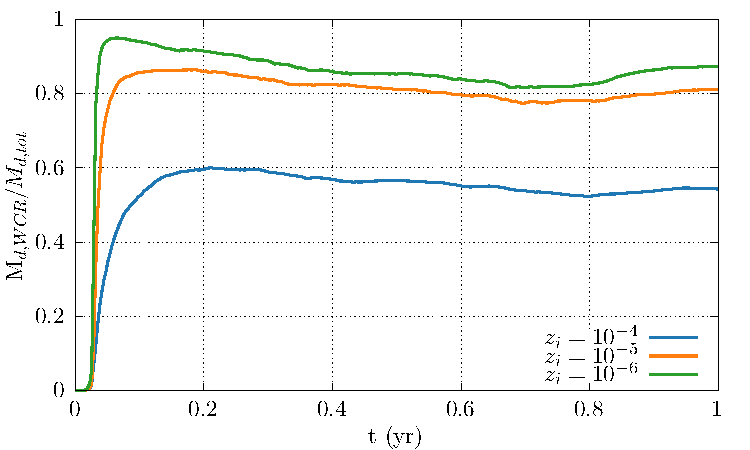
\includegraphics{assets/a_z_tweaking/wcrratio.pdf}
  \caption[WCR dust fraction testing comparison]{A comparison of the WCR dust fraction ($\mass\rms{WCR}/\mass\rms{tot}$) over the course of a simulation with WR98a properties. As $z_i$ deceases the amount of dust produced outside of the WCR decreases significantly. This is consistent across all grain sizes, and does not result in a significantly increased amount of dust.}
  \label{fig:aztwek_wcrrat}
\end{figure}

\begin{figure}[ht]
  \centering
  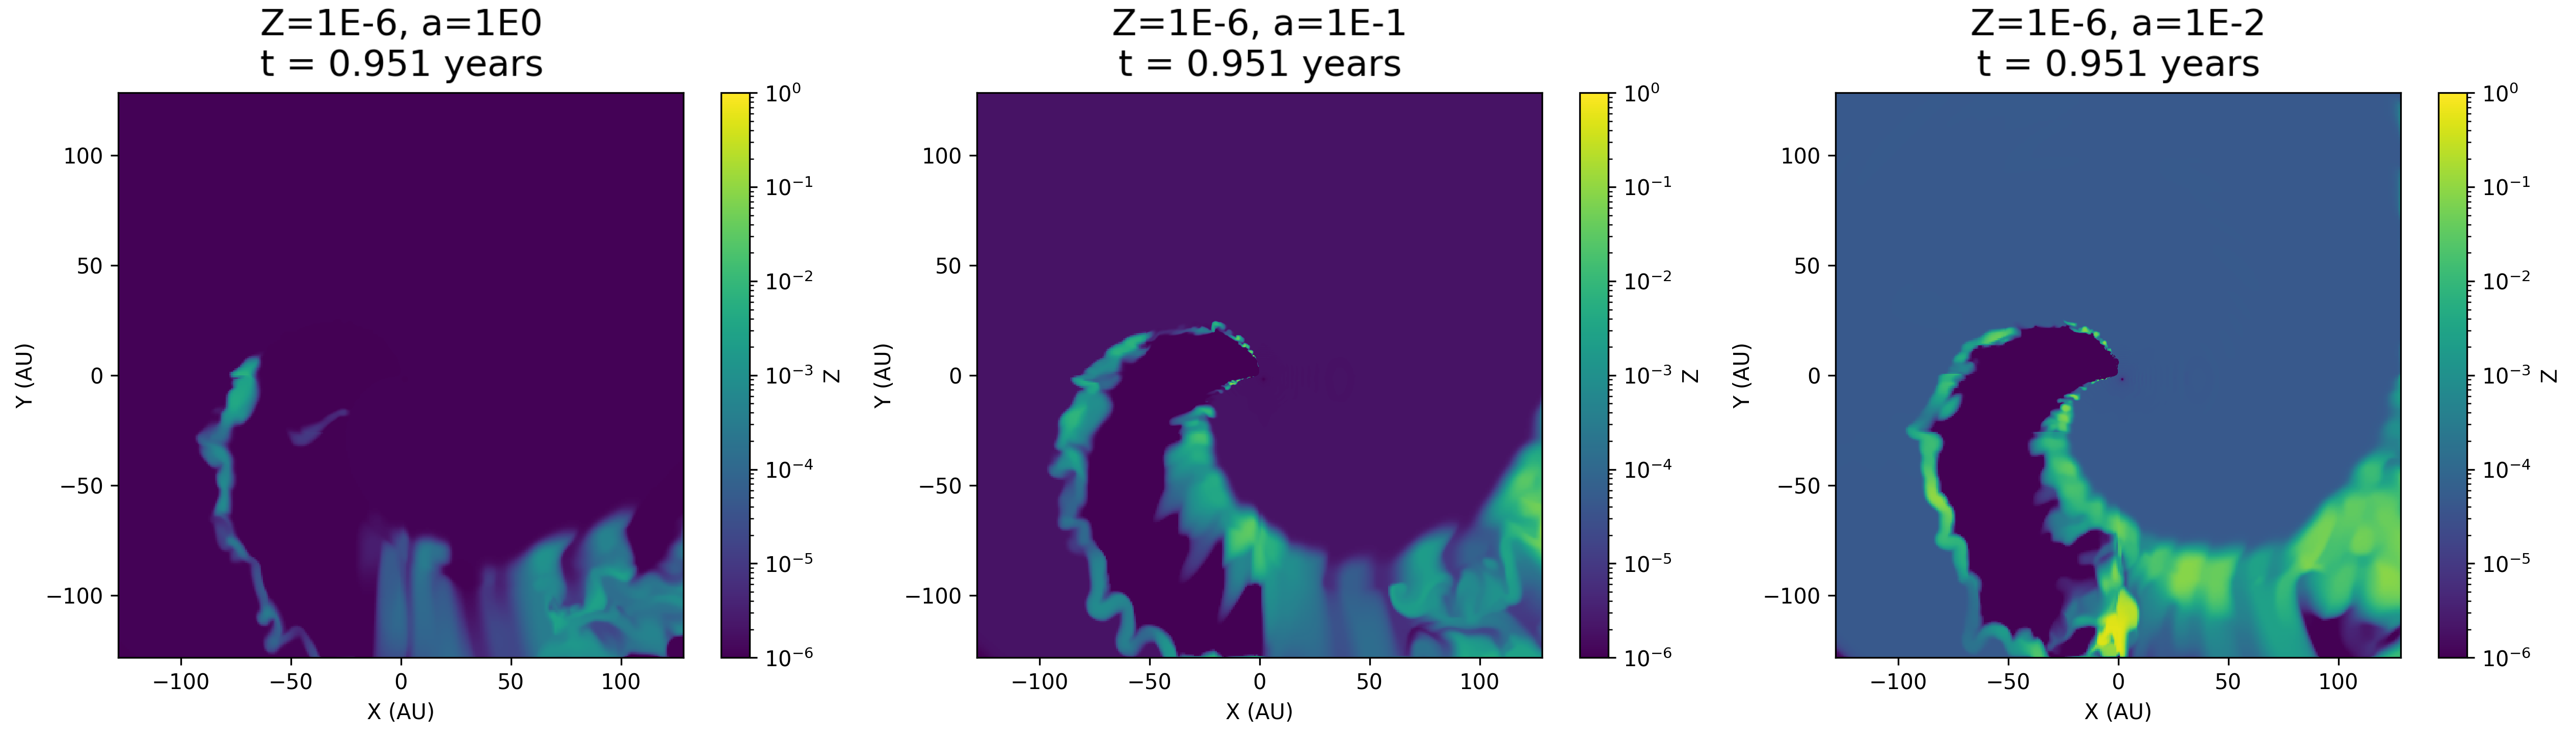
\includegraphics[width=\linewidth]{assets/a_z_tweaking/zconcat.png}
  \caption[$z_i$ testing]{A comparison of WCR dust distribution when $a_i$ is varied in a system with WR98a parameters. Dust yield increases significantly if a smaller, realistic initial grain size is chosen.}
  \label{fig:azweak_img}
\end{figure}

\begin{figure}[p]
  \centering
  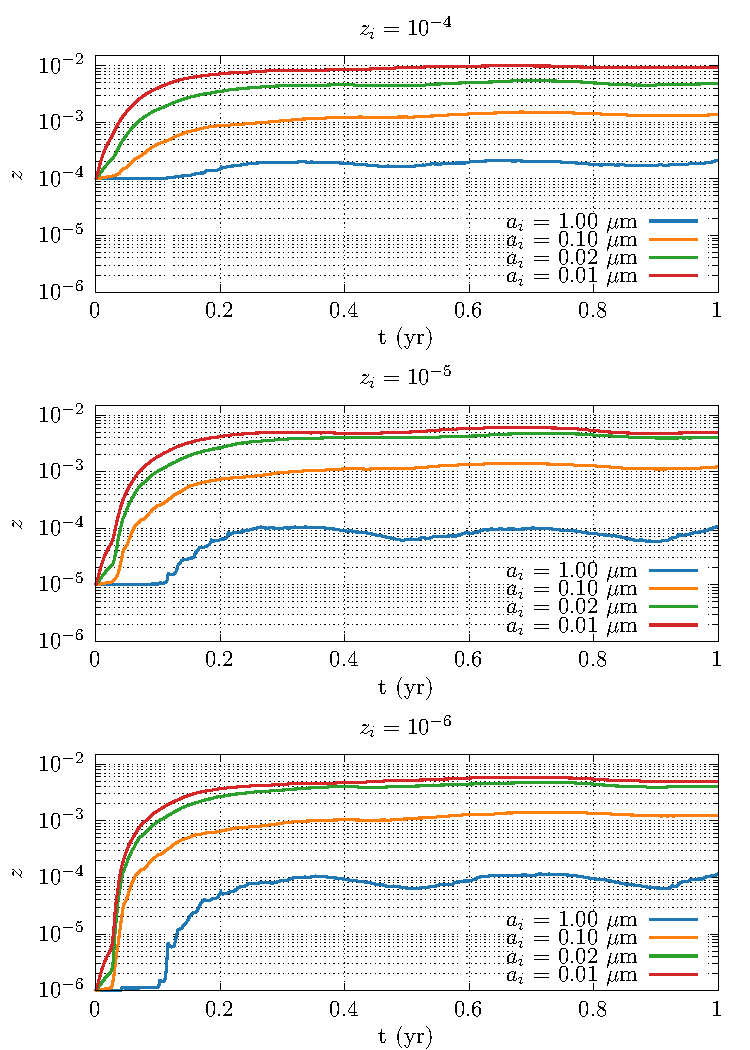
\includegraphics{assets/a_z_tweaking/z.pdf}
  \caption[$z_i$ and $a_i$ parameter tweaking]{A comparison of $z$ over the course of a simulation with WR98a properties, $z_i$ and $a_i$ are varied for each simulation. We find that dust yield increases significantly if a smaller, realistic initial grain size is chosen. Varying $z_i$ does not result in a corresponding change in dust yield.}
  \label{fig:azweak_z}
\end{figure}

Dust is injected into the system in small quantities from the wind remap zone of the WC star.
If we were to describe this mechanism in physical terms, this would be as if refractory carbon grain cores condensed from the WC wind.
Whilst the exact mechanism for initial grain nucleation is not known, this is an ideal first step as it assures that dust grains are present in the post-shock WCR wind.
Another important consideration of this model was for it to be fairly general purpose, and not require significant degrees of initial parameter ``hunting'' in order to simulate a new system.
As such it was decided that the model would operate on as few initial parameters as possible.
% INitial comparisons
Determining the injected scalar values at this remap zone was an important first step, as it was not known how these initial parameters would impact the final dust yield, $\mass\rms{d,f}$, or the dust formation rate, $\mdot\rms{d}$. 
In order to determine the ideal initial parameters, and to determine the sensitivity of the model to it's initial conditions, a series of simulations were conducted using the orbital and wind parameters of WR98a.
The initial grain radius, $a_i$ was varied from \SI{0.01}{\micro\metre} to \SI{1}{\micro\metre}, while the initial dust-to-gas mass ratio, $z_i$ was varied from $10^{-6}$ to $10^{-4}$.
These simulations were run over the course of a week on the ARC4 HPC cluster over 128 cores.
The total elapsed time within the simulation was one year, with the simulation advecting fully to the simulation extent of $100\times 100 \times 10 \, \si{\au}$ in around \SI{0.1}{\year}.
Whilst the results of \textcite{lauRevealingEfficientDust2021} had not been published at this time, a final dust-to-gas mass fraction of $\sim 1\%$ was assumed to be an ideal starting point for a model of WR98a.


As can be seen in Fig. \ref{fig:azweak_img}, we find that decreasing $a_i$ creates a much defined WCR, at the cost of increasing dust outside of the WCR.
Dust formation occurs where expected, on the WC edge of the WCR, with the bulk of dust formation occurring within a short distance from the apex of the WCR shock.
Therefore, we must aim for a small grain radius, and not start with large grains.
Additionally, \textcite{zubkoPhysicalModelDust1998a} notes that the initial dust grain nuclei are expected to be extremely small, on the order of \SI{5}{\angstrom}, and rapidly grow to \SI{100}{\angstrom} through interactions of small, charged grains with impinging carbon ions.
This is expanded on in Fig. \ref{fig:aztwek_wcrrat}, where we find that changing $z_i$ significantly affects the amount of dust produced in the WCR compared to the total dust yield.
As we do not observe significant quantities of dust being produced outside of the WCR, we prioritised a small value of $z_i$, so long that it does not influence dust yields.
Finally, Fig. \ref{fig:azweak_z} shows that changing $z_i$ does not affect the total dust yield significantly, and is far more sensitive to changes in $a_i$.
We can therefore discern from these previous two results that $z_i$ should be kept to a fairly small value.

The other parameter, $z_i$, was found to not effect
Overall, it was found that we could reduce the effective initial parameter space of dust in the wind to a single value, $a_i$, which was found to operate best when kept at realistic values.
After this preliminary parameter space exploration, an $a_i$ of \SI{50}{\angstrom} and a $z_i$ value of $10^{-8}$ were settled on.
Whilst these initial parameters were based on an extrapolation of our test data, these initial values were found to be more than adequate.
Other dust injection mechanisms were considered for this project, such as injecting dust into the apex of the WCR.
However, these were found to give inconsistent results when initially tested in the \mg{} hydrodynamical code.

\subsubsection{Assumptions \& limitations}
\label{sec:bidmasassumptions}
\label{sec:bidmaslimitations}

From this we can determine further assumptions for our dust model.
% Number density
We assume that the number density, $n\rms{d}$, is constant throughout the simulation, which is calculated based on the initial grain radius, $a_i$, and initial dust-to-gas mass ratio, $z_i$, injected into the simulation from the primary star.
% Limitations due to this
Because of this, we therefore assume that the net rate of grain shattering and grain agglomeration is zero.
Additionally, the dust number density may not be correctly calculated, which can affect the rate of cooling.
% Multiple grain sizes and coupling
Additionally, we also assume that there is little variation between grain size within the numerical cell.
% Limitations due to this
Whilst other models assume that dust grains are coupled through a drag force, it was found that the dust was effectively coupled to the wind as if it was co-moving (Section \ref{sec:hendrixmodel}).
This may however prevent significant dust mixing in the immediate post-shock region, due to the increased inertia of the dust grains compared to the gas.
% Grain-grain collision
As a single grain size is assumed, dynamics between grains of different sizes, such as grain agglomeration cannot be accurately simulated.
% Fixes
These issues could be addressed with a multi-scalar or multi-fluid model, which is a potential future feature of this project.

All grains in the simulation are assumed to be circular, with a volume, $V\rms{gr}$, of $4/3 \pi a^3$ and a mass, $m\rms{gr} = V\rms{gr} \rho\rms{gr}$, where $\rho\rms{gr}$ is the grain bulk density.
As we assume all dust grains in the simulation are composed of amorphous carbon, we assume a grain density of \SI{3}{g.cm^{-3}}, which is on the upper end of densities expected for amorphous carbon
\parencite{bhattaraiEvolutionAmorphousCarbon2018}.

\subsubsection{Dust cooling}

Dust cooling is handled within the cooling loop, and functions by removing energy from a cell of the simulation.
The gas is assumed to be optically thin to infrared, and is therefore removed from the simulation without re-adsorption.
The emissivity of the grains at the current temperature and radius, $\Lambda(a,T)$, is calculated for each cell, and the rate of energy loss due to dust emission is calculated such that:

\begin{equation}
  \frac{dE}{dt} = n\rms{T} n\rms{d} \Lambda\rms{d}(T,a),
\end{equation}

\noindent
Where $n\rms{T}$ is the total gas number density and $n\rms{d}$ is the dust number density.
Dust cooling, as well as the optimisations needed to run quickly in a numerical simulation, is discussed in significantly more detail in Section \ref{sec:dustcoolingmodel}.

\subsubsection{Dust evolution}

Once the energy loss due to dust emission has been calculated, the growth rate and destruction rate for dust grains in each cell is calculated.
The code loops through every cell in the simulation, first calculating the average mass of the wind in the cell, $\mu$:

\begin{equation}
  \mu = C \left(2 X\rms{WR} + \frac{3}{4} Y\rms{WR} + \frac{1}{2} Z\rms{WR} \right)^{-1} + (C-1) \left(2 X\rms{OB} + \frac{3}{4} Y\rms{OB} + \frac{1}{2} Z\rms{OB} \right)^{-1} ,
\end{equation}

\noindent
where $C$ is the wind ``colour'', and $X,Y,Z$ are the individual wind hydrogen, helium and metal mass fractions, respectively
\parencite{mihalasStellarAtmospheres1978}.
The cell temperature is then calculated using the ideal gas law:

\begin{equation}
  T = \frac{\mu P\rms{g}}{\rho\rms{g} k\rms{B}},
\end{equation}

\noindent
where $P\rms{g}$ is the gas pressure and $\rho\rms{g}$ is the gas density.
Based on the gas temperature, we determine which dust processes occur.
For temperatures above $10^6 \, \si{K}$, dust destruction occurs, while at temperatures below \SI{1.4e4}{K} dust growth occurs instead.
As the dust grains are assumed to be spherical, we can model dust growth and destruction in a unified manner, corresponding to a change in grain radius.
In the case of dust destruction, ions sputter off atoms from the surface of the dust grain, wearing the grain evenly over time, while in the case of accretion, low velocity collisions cause atoms to stick, growing the grain evenly.

For both processes we find a change in the grain radius of $da/dt$, which can be extrapolated to find the rate of change in dust density with the formulae:

\begin{subequations}
  \begin{align}
    \frac{dV\rms{gr}}{dt} & = 4 \pi a^2 \frac{da}{dt} ,\\
    \frac{dm\rms{gr}}{dt} & = \rho\rms{gr} \frac{dV\rms{gr}}{dt} ,\\
    \frac{d\rho\rms{d}}{dt}   & = n\rms{d} \frac{dm\rms{gr}}{dt} ,
  \end{align}
\end{subequations}

\noindent
where $dV\rms{gr}/dt$ is the rate of change in the dust grain volume and $dm\rms{gr}/dt$ is the associated change in dust grain mass.
To simulate dust growth due to grain-gas accretion we use a method from \textcite[Ch.~9]{spitzerPhysicalProcessesInterstellar2008}.
Carbon atoms accrete onto a dust grain at a constant rate, resulting in a change in radius such that:

\begin{equation}
  \label{eq:dustgrowthradiuschange}
  \frac{da}{dt} = \frac{\xi \rho\rms{C} w\rms{C}}{4\rho\rms{gr}} ,
\end{equation}

\noindent
where $\xi$ is the grain sticking factor, $\rho\rms{C}$ is the density of carbon in the wind ($\rho\rms{C} = \rho\rms{g} X(C)$, where $X(C)$ is the carbon mass fraction), and $w\rms{C}$ is the RMS velocity of ($w\rms{C} = \sqrt{3k\rms{B}T / 12 m\rms{H}}$).
Throughout this thesis we use a grain sticking factor of 0.1, though in the case of ionised gas, this value can be as high as 1.
From Eq. \ref{eq:dustgrowthradiuschange} we can derive a corresponding rate of change in the dust density:

\begin{equation}
  \frac{d \rho\rms{d,acc}}{dt} = \pi \xi \rho\rms{C} w\rms{C} n\rms{d} a^2.
\end{equation}

\noindent
Dust destruction is carried out through the \textcite{draineDestructionMechanismsInterstellar1979} prescription.
We estimate an amorphous carbon grain \SI{1}{\micro\metre} to have a lifespan, $\tau\rms{d}$, of \SI{3e6}{\year}.
As described in \textcite{draineDestructionMechanismsInterstellar1979}, with additional work by \textcite{tielens_physics_1994} and \textcite{dwekCoolingSputteringInfrared1996}, this grain lifespan is dependent on the gas density, $n\rms{g}$, as well as the grain radius, taking the form:

\begin{equation}
  \tau\rms{d} = \frac{a}{da/dt} \approx \num{3e6} \frac{a}{n\rms{g}} \, \si{\year} ,
\end{equation}

\noindent
We can rearrange this equation to find a rate of change in grain radius of $da/dt = a / \tau\rms{d}$.
Finally, we find an associated rate of change in the dust density of:

\begin{equation}
  \frac{d \rho\rms{d,sput}}{dt} = -4 \pi n\rms{d} \frac{\rho\rms{gr} a^3}{\tau\rms{d}} = -4\pi n\rms{d} \frac{\rho\rms{gr} n\rms{g} a^2}{\num{3e6}},
\end{equation}

\noindent
In order to find the total change in the dust density, $\Delta \rho\rms{g}$, and the grain radius, $\Delta a$, we perform a Euler integration over the simulation timestep, $\Delta t$:

\begin{equation}
  \Delta x = \int^{t+\Delta t}_{t} \frac{dx}{dt} dt \approx \frac{dx}{dt} \Delta t ,
\end{equation}

\noindent
where $x$ is the quantity being integrated and $t$ is the simulation time.
Whilst a Euler method integration is less accurate than a sub-stepping method or higher-order integration method, this was found to be adequate, as the growth rate of the dust grain was found to be small over a single time step.
After the total change for $\rho\rms{d}$ and $a$ are calculated, the post-step grain radius, $a\rms{new}$, is calculated:

\begin{equation}
  a\rms{new} = a\rms{old} + \Delta a .
\end{equation}

\noindent
Then the post-step dust and gas densities are calculated, with the new dust being subtracted from the fluid:

\begin{subequations}
  \begin{align}
    \rho\rms{d,new} & = \rho\rms{d,old} + \Delta \rho\rms{d} , \\
    \rho\rms{g,new} & = \rho\rms{g,old} - \Delta \rho\rms{d} . 
  \end{align}
\end{subequations}

\noindent
Finally, the new dust-to-gas mass ratio can be calculated from the new dust and gas densities:

\begin{equation}
  z\rms{new} = \frac{\rho\rms{d,new}}{\rho\rms{g,new}} . 
\end{equation}

\noindent
These new scalar values then overwrite the previous scalar values.
Passive scalars in \athena{} are stored in the following arrays for a scalar species \texttt{N} in a meshblock with indices \texttt{i,j,k}:

\begin{itemize}
  \item \texttt{pmb->pscalars->r(N,i,j,k)}: Primitive variables between \texttt{0.0} and \texttt{1.0}.
  \item \texttt{pmb->pscalars->s(N,i,j,k)}: Conserved variables between \texttt{0.0} and \texttt{rho}, the conserved cell density.
\end{itemize}

\noindent
These values have to be updated simultaneously, and occurs at the end of each iteration of the main processing loop such that:

\begin{lstlisting}[language=c++]
  // Update primitive scalars
  pmb->pscalars->r(1,k,j,i) = z_new;  // Update z primitive
  pmb->pscalars->r(2,k,j,i) = a_new;  // Update a primitive
  // Update conserved scalars 
  pmb->pscalars->s(0,k,j,i) = col   * rho_new;  // Update colour conserved
  pmb->pscalars->s(1,k,j,i) = z_new * rho_new;  // Update z conserved
  pmb->pscalars->s(2,k,j,i) = a_new * rho_new;  // Update a conserved
\end{lstlisting}

\noindent
\athena{} automatically re-scales scalar values lower than \texttt{0.0} or greater than \texttt{1.0} or \texttt{rho} (depending on the variable type) at the end of each time-step\footnote{This method also limits the grain size to a maximum radius of \SI{1}{\micro\metre}, but growth of this level outside of testing - where the grain radius was stored in centimetres - was never observed.}.

\subsection{Contemporary dust Models}

At the time of writing, there has been no research conducted that has accomplished all three of the following criteria:

\begin{enumerate}
  \item Models a CWB system using a numerical simulation.
  \item Implements a dust model inside this numerical simulation.
  \item Simulates multiple features such as dust accretion, sputtering and radiative cooling.
\end{enumerate}

\noindent
There are two dust models in particular, however, that should be discussed, as they fulfil some of these conditions.
These are the \textcite{harriesThreedimensionalDustRadiativetransfer2004} and \textcite{hendrix_pinwheels_2016} dust models.
% Ballistic dust model
Research conducted by \textcite{harriesThreedimensionalDustRadiativetransfer2004} involved the simulation of dust emission through a ballistic particle model, with the CWB simulated as a conical region.
Dust of a uniform size of \SI{0.01}{\micro\metre} was used, with the cone being simulated with a radiative transfer model, in order to constrain the dust production rate of the WR104 system through comparison to observations.

\subsubsection{The Hendrix dust model}
\label{sec:hendrixmodel}

Perhaps the most similar contemporary dust model is the model described in \textcite{hendrix_pinwheels_2016} - as this model is concerned with simulating the dynamics of dust within a CWB.
This is not to say that these models are identical, of course, as the Hendrix model explores how dust spreads throughout the WCR of WR 98a, in order to compare with observational data using radiative transfer code.

% Differences between models 

The main differentiating factors between this model and our model are the driving mechanism and dust evolution.
In the Hendrix model dust is modelled as a separate fluid, with an Epstein drag function between the wind and dust fluids; this method allows for dust kinematics that aren't implicitly co-moving.
This is a more accurate method of modelling dust, however it requires significantly more processing time and is much more difficult to implement, requiring a numerical code that supports multiple fluids.
At the start of this PhD this was considered but eventually rejected due to time constraints.

However, the Hendrix model has limitations that this model does not have, this is because the purpose of the Hendrix model is to analyse the distribution of dust within a CWB system, rather than to model the evolution of the dust itself.
To this end, the Hendrix model does not calculate dust growth or destruction, and only uses a single small grain size, with the dust-to-gas mass ratio calculated based on observations of the target system, WR98a.

\subsection{Future dust models}

% Future work, adopt multi-fluid model?

Due to time constraints and limitations in the code in use, only a limited set of mechanisms for dust evolution were included in this projects simulations.
While the \bidmas{} model represents an interesting start for the modelling of dust grains in colliding wind binaries, future models could implement more complex models which incorporate additional destruction and growth mechanisms, as well as a multiple dust grain sizes.

A multiple grain size scalar model could be used to more accurately measure the growth of dust grains, rather than a single average grain size.
This would be more difficult to implement than a single model but would be able to estimate grain-grain collision, and better estimate dust growth and destruction rates.
\athena{} and MG both have issues with a large number of scalars, as such both numerical codes may require significant modification to cope with this.
A multi-fluid model with dust being physically simulated rather than assumed to be perfectly co-moving would be an ideal next step.
Multiple grain size distributions could also be modelled in a similar way to the proposed multi-scalar model, however the kinematics of the dust grains could also be simulated separately.
% Mixing factors
The increased inertia of more massive dust grains could result in the kinematics of the dust flow diverging from the co-moving assumption.
To that end, a successor dust model would adopt a multi-fluid and drag function method, which was considered but not included for the sake of time.
This multi-fluid model would also allow for more physically accurate simulation of grain-gas and grain-grain interactions, as the collision velocities would be exactly calculated rather than estimated through bulk motion properties.
High speed collision of gas on dust grains in the immediate post-shock environment could also shatter grains, though modelling this as well as spalling of particles in the wind through the dust grains would be complex to simulate. 

Furthermore, additional mechanisms for dust destruction, such as through photodissociation and sublimation could also be implemented, the implementation of these could be used to determine the effectiveness of the WCR in protecting nascent, still forming dust grains.

% Better dust nucleation model

The initial grain nucleation model could also be improved, injection of extremely small grains into the simulation through the stellar remap zones was chosen as the underlying chemical process for formulation of these dust grains is poorly understood at the time of writing.
% Current model not too bad, strong dependence on a but z does not change much, being dependent on a single parameter not too bad
The small grain nucleation model was also found to be only dependent on the initial grain radius, $a_i$, whilst changing the amount of grain nuclei in the WR wind does not change the amount of dust produced.
As such the simulations are currently bound by a single input parameter, which can be constrained based on what is currently understood about dust grain accretion.
% Difficulty in picking initial parameters for more complex model
A more complex model may require additional parameters, and as such could be highly dependent on these initial parameters, as such, another round of initial parameter hunting would be required.

% Comparison with observational results

\begin{figure}[ht]
  \centering
  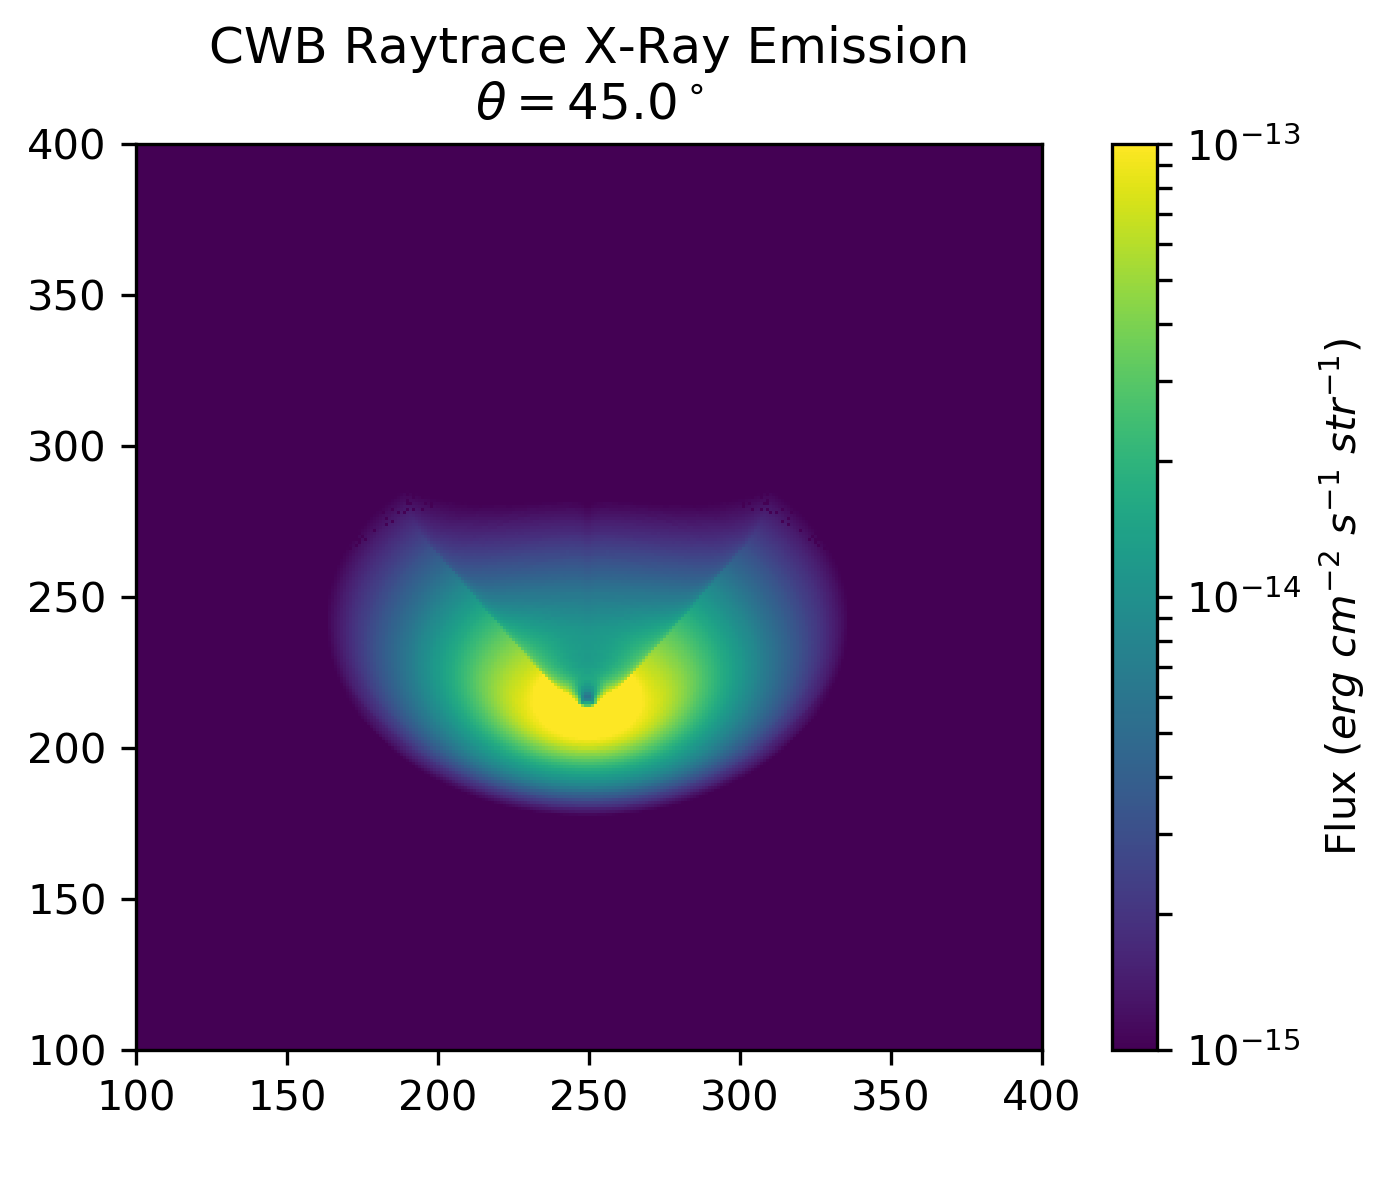
\includegraphics[width=4in]{assets/ray/cwb-raytrace-045.0.png}
  \caption{X-ray radiative transfer image from \SI{0.1}{\kilo\electronvolt} to \SI{10.0}{\kilo\electronvolt} of a test CWB system with a momentum ratio of $\eta = 0.01$ inclined at $\phi = 45^\circ$ from the obesrver at a distance of \SI{1}{\kilo\parsec}. Radiative transfer was performed on an in-house code, which was to be modified to support dust emission.}
  \label{fig:inhousert}
\end{figure}

Another avenue of future research would be performing a radiative transfer simulation upon a fully advected system, in order to compare with observational results.
Whilst some initial tests were performed with in-house x-ray emission code that was to be modified to support dust emission (Fig. \ref{fig:inhousert}).
Using other radiative transfer codes such as \texttt{HYPERION} were also considered \parencite{robitailleHYPERIONOpensourceParallelized2011}, but this was abandoned due to time constraints from changing hydrodynamical codes from \mg{} to \athena{}.
Radiative transfer modelling was performed by \textcite{hendrix_pinwheels_2016}, with the resultant images emulating the sensitivity and angular resolution characteristics of UKIRT, Keck and ALMA (figure \ref{fig:hendrix-synthetic}).

\begin{figure}[ht]
  \centering
  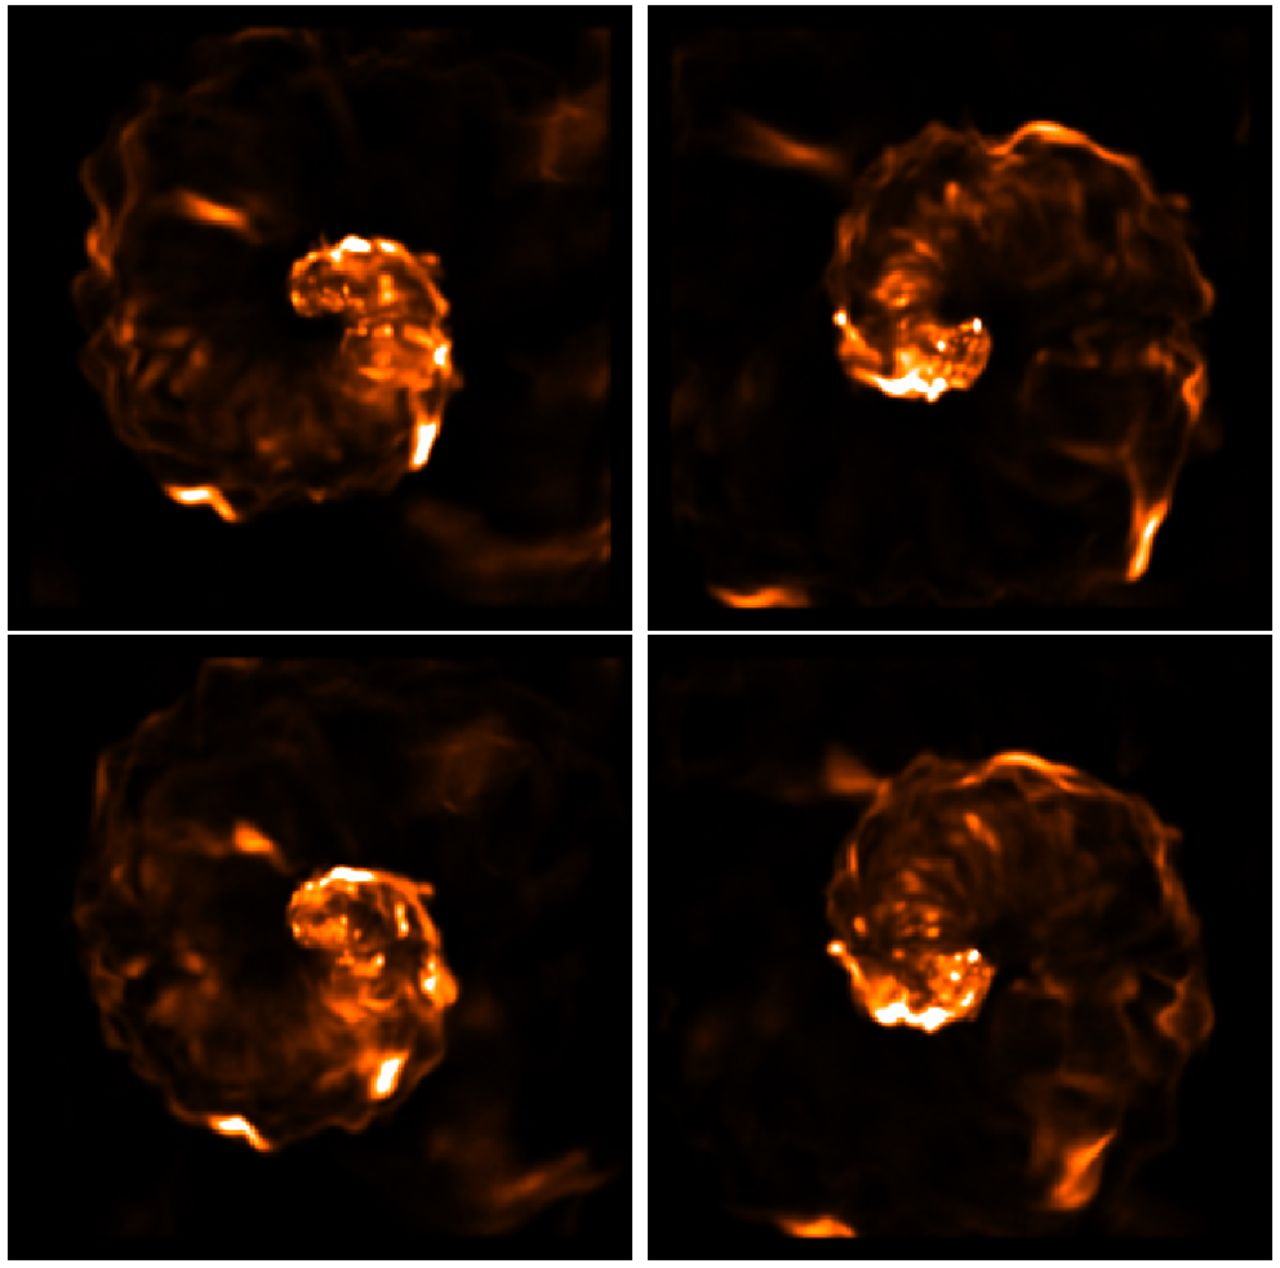
\includegraphics{assets/hendrix-synthetic-observation.jpeg}
  \caption[\textit{Radiative transfer images of WR98a \parencite{hendrix_pinwheels_2016}}]{Synthetic images of WR 98a emulating the capabilities of ALMA using a radiative transfer model, reproduced from \textcite{hendrix_pinwheels_2016}.}
  \label{fig:hendrix-synthetic}
\end{figure}
